\chapter{saMsakxqqtAyoVgada parxshAnxvaLige utatxra}

\noindent
{\large\bf saMsakxqqtAyoVgada parxshenxgaLige utatxrisabeVkAda parxkaraNa}\label{page19}
\medskip

\noindent
(saMsakxqqta BASeya vAyxsaMgavananxBivaqdidhxpaDisalu, hiMdomemx saMsakxqqtAyoVga\-voMdu keVMdarx sakAR\-radiMda rUpugoMDu, aneVka vidAyxsaMsethxgaLige aBipArxya saMgarxhakAkxgi (AyoVgavu) parxshAnxvaLiyanunx kaLuhisi yoVgayx utatxragaLanunx bayasitutx. A samayadalilx naMjanagUDu tAlUlxku heDatale keSxVtarxdalilx aSATxMgayoVgavijAcnxnamaMdirada keVMdarx kAyARlayavu tananx kAyaRgaLanunx naDesutitxtutx. vijAcnxna\-maMdirakUkx  parxshAnxvaLiyu baMdidadxriMda maMdirAdhayxkaSxrAda shirxV shirxVraMga mahAguruvu anugarxhisida viSayagaLanunx (saMsakxqqtiVkarisi) meVlakxMDa AyoVgakekx kaLuhisalAgitutx. adanunx ililx muMdiDalAgide. {\rm 13-02-1956})  

\bigskip

\noindent
{\large\bf vidAyxmUlanAda hayagirxVvana samxraNe}\label{page19}
\medskip

\begin{shloka}
vishovxVtitxVNaRsavxrUpAya cinamxyAnaMdarUpiNeV |\\\label{19}
tuBayxM namoV hayagirxVva! vidAyxrAjAya viSaNxveV ||
\end{shloka}

\begin{shloka}
jAcnxnaM teV haMsavijAcnxnamidaM vakASxyXmayxsheVSataH |\\\label{19}
yadfjAcnxtAvx neVha BUyoV\char'263 nayxtf jAcnxtavayxmavashiSayxteV ||\\
\hfill Ba. giV
\end{shloka}

\begin{figure}[H]
\centering
{\includegraphics[scale=.19]{0019.eps}}
\caption{jaya vishavxBArati !}
\end{figure}

\noindent
{\large\bf BArata padada athaR vivaraNe}\label{20}
\medskip

\begin{shloka}
BAti saveVRSu veVdeVSu ratiH saveVRSu jaMtuSu |\\\label{20a}
taraNaM savaRtiVthARnAM teVna BAratamucayxteV ||
\end{shloka}

\medskip
\noindent
{\large\bf deVva BASe-saMsakxqqtada baagege shuBAshaMsane}\label{20b}
\medskip

\begin{shloka}
yAvadasitx tarxyiV loVkeV catumuRKamuKoVdaBxvA |\\\label{20c}
yAvadAvx rAmacaritaM vAlikxVki-kavi-citirxtamf ||
\end{shloka}

\begin{shloka}
kaSxraMtayxmaqtadhArA vA yAvadf vAyxsasayx sUkatxyaH |\\
vAgedxVvAyx varaputarxsayx kALidAsasayx vA giraH ||
\end{shloka}

\begin{shloka}
tAvadeVSA deVvaBASA deVviV sAthxsayxti BUtaleV |\\
yAvacacx vaMshoV\char'263 sAtxyXyARNAM tAvadeVSA dhurxvaM dhurxvA ||
\end{shloka}

{\medskip
\noindent
{\large\bf saMsakxqqtAyoVgakekx kaLuhisida viSayagaLa anukarxmaNike}}\label{20d}
\begin{itemize}
\item[{\rm1.}] parxsAtxvane
\item[] utatxragaLu
\item[{\rm 2.}] e. viBAga
\item[{\rm 3.}] bi viBAgada BUmike.
\item[{\rm 4.}] bi viBAgada utatxragaLu.
\item[{\rm 5.}] si viBAga.
\item[{\rm 6.}] Di viBAga.
\item[{\rm 7.}] upasaMhAra
\end{itemize}

{\medskip
\noindent
{\large\bf savaRvidAyxmUlavAda satayxda samxraNarUpavAda maMgaLa}}\label{20e}
\begin{itemize}
 \begin{shloka}
\item[{\rm 1}] IshAnaH savaRvidAyxnAmiVshavxra: savaRBUtAnAmf |\\\label{20f}
barxhAmxdhipati barxRhamxNoV\char'263 dhipati barxRhAmx shivoV meV asutx sadAshivoVmf ||
\item[{\rm 2}] QucoV \char'263 kaSxreV parameV voyxVmanf |\\\label{21}
yasimxnf deVvA adhivishevxV niSeVduH |\\
yasatxnanx veVda kimaqcA kariSayxti? |\\
ya itatxdivxdu satx imeV samAsateV ||
\item[{\rm 3}] vijAcnxneVnA\char'263\char'263 tAmxnaM veVdayati |\label{21} 
\item[{\rm 4}] na hi jAcnxneVna sadaqshaM pavitarxmiha vidayxteV ||\label{21}
 \item[{\rm 5}] QuSiBibaRhudhA giVtaM CaMdoVBiviRvidheY: paqthakf |\\\label{21}
barxhamxsUtarxpadeYshecxYva heVtumadiBxviRnishicxteY: ||
\item[{\rm 6}] adhAyxtamxjAcnxna nitayxtavxM tatatxvXjAcnxnAthaRdashaRnamf |\\\label{21}
Etatf jAcnxnamiti porxVkatxmf ajAcnxnaM yadayoV\char'263 nayxthA ||
\end{shloka}
\end{itemize}

%~ \begin{itemize}
 %~ \begin{shloka}
 %~ \item[{\rm 5}] QuSiBibaRhudhA giVtaM CaMdoVBiviRvidheY: paqthakf |\\\label{21}
%~ barxhamxsUtarx padeYshecxYva heVtumadiBxviRnishicxteY: ||
%~ \item[{\rm 6}] adhAyxtamx jAcnxna nitayxtavxM tatatxvXjAcnxnAthaRdashaRnamf |\\\label{21}
%~ Etatf jAcnxnamiti porxVkatxM ajAcnxnaM yadayoV\char'263 nayxthA ||
%~ \end{shloka}
%~ \end{itemize}

{\medskip
\noindent
{\large\bf saMsakxqqtAyoVgada kArayxda parxshaMseyoMdige vijAcnxpane}}\label{page21}

\bigskip

{\centerline{\large\bf{shirxV sadugxraveV namaH}}}

\medskip

satayx-jAcnxna-anaMtavAda suKada mUlaneleyAgiruvaMthadAgidadxrU saha, iMdinavarAda\- namamx kaNiNx\-niMda dUravAgiruva (daqSiTx goVcaravAgadiruva) sanA\-tanAyaR BAratiVya saMsakxqqti matutx nAgari\-kategaLiMda {\rm (Civilization)} samaqdadhx\-vAgiruva saMsakxqqtaBASeya bagege rASaTxrXda parxjegaLalilx yathAthaR\-vAda arivu mUDuvaMte mADaloVsuga hoNeyanunx hotutx mahAyajacnxrUpavAda I utatxma\-vAda kAyaRdalilx kaMkaNabadadhxrAgaliruva saMsakxqqtAyoVgada sadasayxralilx swhAdaRpUNaRvAda vijAcnx\-pane\-gaLu.

{\medskip
\noindent
{\large\bf saMsakxqqtada bagegx arivu mUDisuva kArayx nilalxdeV beLeyabeVku}}\label{page21}
\medskip

\noindent
jiVvanada paramalakaSxyX (guri), adakAkxgi ADikoLuLxva mAtukate, matutx adanunx kirxyeyalilxLisuva naDe ivugaLalilx parasapxra sAmarasayx matutx sAmaMjasayxgaLilalxdaMtAgi, aMdhAnukaraNa paraMpareyalilx sikikx\-koMDu muLugutAtx rASiTxrXVya parxjegaLelalxrU adhoVgatiyalilx sAgutatxliruva I desheyalilx, I riVti saMpadaBx\-ritavAda saMsakxqqta BASeya arivu janatege neYjavAgi-satayxvAgi dorakuvaMtAgabeVkeMduMTAgiruva manasusx maraLugADinaMtAgiruvaMtaha I rASiTxrXVya jiVvanadalilx niVrina bugegx\break\-yanunx kANuva cihenx\-yaMte toVruvudAgide. Adare hiVge toVridudx bisilu kudure(maqgamariVcike)yAgibiDadeV, jiVvi\-gaLa jAcnxna pipAseyanunx nija\break\-vAgiyU niVgisabalalx ashoVSayxvAda amaqta-jaladhAreyAgi hari\-yuva jAcnxna\-gaMgeyAdare mAtarx, BAratiVya parxjegaLa sherxVya: perxVyasusxgaLiMda tuMbida pUNaR\-jiVva\-navu matetx sAdhayxvAdiVtu.

{\medskip
\noindent
{\large\bf BAratiVya videyxkalegaLa guri}}\label{page22}
\medskip

\noindent
namamx deVha, mAtu, manasusx, iMdirxyagaLu, budidhx, parxkaqti matutx Atamx ivelalxkUkx heVge parasapxra atayxMta nikaTavAda saMbaMdhavidudx jiVvanavu naDeyutitxdeyoV, aMteyeV jAcnxna-vijAcnxna cakuSxSakxrAda sanAta\-nAyaR-BArata mahaSiRgaLu taMdaMtaha, `saMsakxqqti matutx nAgarikate' gaLanonxLagoMDa catu\-SaSxSiTx(64) videyx (kale)gaLigU matutx vishavxgoVLoVtatxra dhurxvadalilx kUTasathxnAgi beLaguva A paraMjoyxVti\-sisxgU saha aSeTxV nikaTasaMbaMdhavide. aSeTxV
alalxdeV A videyxgaLelalxvU A paraMjoyxVtiya anuBavada kaDege loVka\-vanonxyuyxva BAratoVtatxramuKigaLU Agive. {(\rm Mariner's Compass)}

{\medskip
\noindent
{\large\bf vijAcnxnamaMdirada kArayxgaLu hAgu Ashaya}}\label{page22}
\medskip

\noindent
iMdu kaNamxreyAgiruva aMtaha BAratiVya saMsakxqqti nAgarikategaLa viSayadalilx veYjAcnxnika\-vAda shoVdhane matutx parxyoVgagaLanunx yathAyoVgayx naDesi, avugaLiM\-dodagi\-baMda sAvxnuBavagaLa AdhArada meVle bagege harida viSayagaLanunx avugaLa javAbAdxri, adhikAri, kAla-deVsha-vataRmAnagaLu ivelalx\-vananxnu\-sarisi, aMteyeV yathAshakitx yathAkAlAvakAsha loVkada muMdiDuvudU vijAcnxna maMdirada Ashaya\-vAgide.

{\medskip
\noindent
{\large\bf vijAcnxnamaMdirada hinenxle}}
\medskip

\noindent
keVvala pusatxka pAMDitayxdalilxyeV niMtu, (pusatxkagaLalilx kaMDaMtaha) shAsatxrX vAkayx matutx padagaLanenxV meluku hAkikoLuLxtAtx caviRtacavaRNa mADuvudariMdaleV\break sanAtanAyaR BAratiVyara shAsatxrXgaLi\-gelAlx EkeYka lakaSxyXvAda badukina (satayx\-vasutxvina) rasAnuBavavAgadu. A padAthaRda (satayxvasutxvina) jAcnxnAnu\-BavagaLa beLakinalilx shAsatxrXgaLananxthaRmADikoMDAga tAneV namamx 
savARMgiVNa vikAsarUpavAda A parama\-shAMti\-yanAnxsAvxdisalu sAdhayxvAdiVtu. I KacitavAda aBipArxyavanunx, parxyoVgAtamxkavAda nishacxya hoMdida\- vijAcnxnamaMdiravu dhiVravANiyiMda heVLahoraTu `na shAmayxti vinApAnaM vAyxdhirwSadha\-shabadxtaH'\label{25} eMdu daqDhavAgi sArutatxde. (auSadhavanunx pAnamADadeV `auSadhi auSadhi' eMba sadidxniMda mAtarx\-veV vAyxdhiyu aDagalAradu.)

{\bigskip
\noindent
{\large\bf diviBuvigaLa seVtu-BArata saMsakxqqti}}\label{page23}
\medskip

\noindent
vishavxda saqSiTxge mUlavAdaMtaha A paramashAMtiya tANavanenxV tamamx daqSiTxge nele\-yanAnxgiTuTxkoMDu (sAdhane mADi), saMpUNaRvAda saqSiTxya meVle oMdu\break siMhAvaloVkanavanunx biVri, naMtara tamamx manasesxMba rathadalilx kuLitu, diviyiMda BuviyavaregU matetx BuviyiMda diviyavaregU saMcarisi, jAcnxna-vijAcnxna\-gaLiMda pUNaRrU taqpAtxtamxrU AdaMtha sanAtanAyaR BArata mahaSiRgaLiMda parxkAsha\-goMDu parxvatiRtavAda saMsakxqqti matutx nAgarikategaLelalxvU, jiVvigaLanunx nirAyAsavAgi aDiDx AtaMkagaLi\-geDeyilalxdaMte BuviyiMda diviyavaregU koMDoyuyxva oMdu sumAgaRvAgide. A hAdiyanunx nAvu hiDidu horaTare, avaru EpaRDisida A yAnavanunx hatitxdare adu hoVgi talapuveDege nAvU talaputetxVve. adeV jiVvanada neledANavU Agirutatxde. adaralilx oMdu gAMBiVyaRvU swMdayaRvU nitayx swKayxvU iruvudu arivAgutatxde. idu tAtitxvXkavAda sithxti.

{\bigskip
\noindent
{\large\bf `BAratiVya saMsakxqqti' - iMdu gata veYBavada palalxvi}}\label{page23}
\medskip

\noindent
hiVgiruvalilx I shAshavxtavAda BUmikeyiMda cuyxtiyanunx hoMdi, AdashaR\-shUnayxvU akaqtayxmayavU Ada sheYshavAvasethxya (neYjavAda ariviniMda dUravAda) modalogxMDu biVLutAtx ELutAtx taDavari\-sutAtx mugagxrisutAtx dikukxkANadeV gotutx\-guri\-gaLilalxdeV Cinanx BinanxvAda kumAgaRgaLiMda tuMbi hoVgiruva iMdina asaMsakxqqta\-vAda bALATadalilx sanAtanArayx-BArata mahaSiRgaLa saMsakxqqti nAgarikategaLiMdodaga\-takakx swMdayARnaMdAnuBavavu heVge tAneV sAdhayxvAdiVtu? yAralilx vicArisi\-darU gataveYBavada palalxviyanunx mAtarx keVLabahudeV horatu sithxtaveYBavakekx elUlx eDeyilalxveMbudu sapxSaTxvAgi tiLiyu\-tatxde.

\newpage

{\medskip
\noindent
{\large\bf ASaR saMsakxqqtiya mamaRvariyadavara vAyxKAyxnagaLa pariNAma}}
\medskip

\noindent
A shAshavxta vasutxvanenxV AdharisikoMDu, adara pArxpitxyanenxV dheyxVyavAgi hoMdi sanAtanAyaR-\-BArata mahaSiRgaLu parxkAshakekx taMda videyx-kale-shAsatxrX ivugaLigU namamx iMdina bALATada anuBava\-gaLigU kiMci\-tAtxdarU sAmarasayxvideyeV? eMbudanunx athaRmADikoLuLxvudU asaMBavavAgide.

BAratiVya saMsakxqqtiyAdarU Enu? eMdu sAvadhAnavAgi shoVdha mADi\-dare, sanAtanAyaR-\- mahaSiRgaLa keY hiDiyalilx (muSiTx) goVpayxvAgi aDagiruva jiVvamaNiyeV Agiruvudu goVcara\-vAgu\-tatxde. A QuSimunigaLa muSiTxyalilx EnaDagideyeMbudanunx heVLalu nAnu muMdu tAnu muMdu eMdu horaTavara kUgeV kUgAgideyAdarU, yAra mAtu managaLU vasutxtatatxvXvanunx muTiTx baru\-titxlalx, matotxMdu pusatxkada mAtananxvalaMbisi hoyodxDutitxdeyeMbudu edudx\break kANutatxde. avaru tamamx muSiTxyalilx mucicxTuTxkoMDidadxrU, yArAdarU pAra\-dashaRkada mUlaka A mareyanunx teredu (tere\-yanunx BeVdisi) noVDi toVrisidAga mAtarx A bagegx itarara arivu mUDiVtu. adu hora\-paTiTxVtu. Adare elalxrU sAru\-vudU saha taMtamamx bALATadalilx kaMDubaruvudara peYki yAvu\-dAda\break\-roMdanenxV QuSi muSiTxyalalxDagiruva jiVvamaNiyeMdu GoVSiSutAtx kAla\break yApane\-mADu\-titxdAdxre. iMdu A bagegx naDeyuva vAyxKAyxnoVpavAyxKAyxna\-gaLelalxvU kuruDanige kuruDaneV dAri toVrisa horaTaMtA\-gide-(aMdheVneYva niVyamAnA yathAMdhAH\label{24})yAdadxriMda IvaRrigU adhoVgatiyeV gati\-yAgide\-yeMdare neYjasaMgatiyadu.

{\medskip
\noindent
{\large\bf yAru mAgaRdashaRkarAgabalalxru?}}
\medskip

\noindent
 AdadxriMda yAru QuSihaqdayavanunx hoMdidavarAgidudx alilxya samAcAra\-vanunx viSaya-parx\-yoVga matutx anuBavagaLige parasapxra viroVdhavanunx tarada parxyoVga vijAcnxnada baladiMda loVkada muMdiDa\-balalxroV, avaru mAtarxveV QuSi saMsakxqqti nAgarikategaLuLaLx jiVvanakekx mAgaRdashaRka\-rAga\-balalx\-reMdu heVLa\-bayasutatxde vijAcnxna maMdira.

{\bigskip
\noindent
{\large\bf BASe-BAvagaLa sAmarasayx}}\label{page24}
\medskip

\noindent
parxkaqta, saMsakxqqta BASeya viSayadalilx eraDu mAtugaLanAnxDabeVkAgide. `BASe' yeMdareVnu? eMba parxshenxge utatxravAgi heVLuvudAdare, BASeyu oDalu-eMdu. oDalige oMdu usiru beVkalAlx \-eMdare, BAvaveV BASeya usiru. BAvada oDaleV BASe. I riVti BAvakUkx BASegU saMbaMdha\-voMdide\-yeMbudu elalxrU ADikoLuLxvudeVnoV nija. loVkadalilx parxtiyoMdu pArxNiyU tananx oLa BAva\-vanunx parxkAshapaDisalu nAnAtarahada sAdhanegaLanunx hoMdiruvudu kaMDu baru\-tatxde. hiVgiruvalilx manu\-Sayxnu tananx BAvABivayxkitxgAgi paDediruva aneVka sAdhane\-gaLa peYki BASeyU oMdu sAdhanavAgide. uLi\-delalx\-kikxMta parxmuKavU Agide. BASeyu vayxkatxvAda vAkAkxdare adakekx mUlavu BAvaveV. udA\-hara\-Nege- roVgi\-yobabxnu naraLutitxruvudanunx gamanisidare, avana nara\-LATavU oMdu BASeyenanx\-bahudu. A BASeyu Enanunx-yAva BAvavanunx horahAkutatxdeyeMdare-\-oLa\-gina veVdaneyanunx. AdadxriMda nara\-LATada BASege oLagina veVdaneyeV BAva\break\-vAgiru\-vudu. A veVdaneya BAvavanunx avana naraLu\-vikeyeV vayxkatxgoLisabalulxdu. yAvudeV mAtanADidarU adariMda A veVdaneyu vayxkatxvAgalAradu. veVda\-nege hoMdikoLuLxva BASe naraLuvikeyeV. hiVge BASe matutx BAvagaLa sAma\-rasayxvirabeVku.

{\medskip
\noindent
{\large\bf amara BASe saMsakxqqta}}
\medskip

\noindent
oDalige (deVhakekx) bele usiriniMda heVgoV, hAgeyeV BASege BAvadiMda mAtarxveV beleyiru\-vudu. I riVti yoVcisi saMsakxqqta BASege belekaTuTxvudAdare, Aga adakekx nijavAda bele. I BASeya BAva\-vAvu\-denunxvu\-dAdare-sanAtanAyaR BArata\-mahaSiRgaLu tamamx susaMsakxqqtavAda aMtaHkaraNadiMda divi\-yalalxnu\-Bavisida amara\-BAvaveV. A amara BAvavanunx vayxkatxpaDisalu-matayxRBUmige taralu baLa\-sida\break BASeyeV saMsakxqqta BASe. amaraBASe-deVvaBASeyenisikoLaLxlu adara hiMde amara BAvavira\-beVku. amara BAvadiMda saMsAkxra hoMdida-pArishudadhxyX\break hoMdida BASeyeV saMsakxqqta BASe. adu BU-savxgaR\-gaLera\-DanUnx oMdugUDi\-suva seVtuveyAgide. hiVge BASeya jiVvavAda amaraBAvavanunx kaLedu\-koMDi\-ruva BASeyAgide iMdu namamx keYge sikikxruva saMsakxqqta BASe. jiVvavanunx kaLedu\-koMDAga maqta\-vAguvu\-daSeTxV. AdadxriMda namamx pAlige dorakiruva BASeyu maqta BASeyAgideyeMdare sari\-yAgutetx. EkeMdare-iSATxru garxMthasahasarx adhayxyana mADiyU AgutitxruvudeVnu? keVvala pada-vAkayx\-gaLa cavaRNe\-yaSeTx. alilxya padAthaRgaLa anuBavavAgaliV adariMda dorakatakakx rasavAgaliV, kiMci\-tAtxdarU haqda\-yakekx iLidilalx. iLiyutitxlalx. 

AyaRmahaSiRgaLu tamamx Atamx, manasusx, budidhx matutx iMdirxyagaLalilx yAva AnaMda rasa\-vanunx tuMbikoMDu, A tuMbuneleyAda amaraBAvavanunx, veVda shAsatxrX-purANeVtihAsagaLa rUpa\-vAda yAva saMsakxqqta vANiyalilx gAna mADi\-daroV, adeV vANiyalilxna veVdashAsAtxrXdi sAhitayxgaLa adhayx\-yana-\-adhAyxpanagaLiMda Iga keVvala gaMTalu oNagutitxdeyeV horatu, A AnaMdarasada taMpA\-galiV amara BAvavAgaliV namamx pAlige ilalx. hiVgAgalu Enu kAraNa? eMdare iMtaha sAhitayx\-kAra\-rAda AyaR\-QuSi\-gaLa\-lilxdadx ASaRvijAcnxnavu namage ilalxdiruvudeV kAraNa. iMtaha duravasethxyalilxdadxrU, bariV duraBi\-mAnavu mAtarx edudx kANutitxde. idelAlx athaRsaMbaMdhavanunx kaLedukoMDa shabAdxDaMbarada veYBava.

{\bigskip
\noindent
{\large\bf BAvadiMda kUDibaMdAga BASege BAvasoVpAnavAguvudu}}\label{page26}
\medskip

\noindent
BagavAnf bAdarAyaNaru athaRdoDane samanavxyavanunx kANada vAkapxrXpaMcadiMda yAvudeV parx\-yoVjanavU dorakalAradeMdu, mahABAratada shAMti pavaR\break 244neV adhAyxyadalilx sapxSaTx\-goLisi\-dAdxre. niVranunx kuDidAga adara taMpu heVge gaMTalinalilx dorakuvudoV hAge sadABxvavuLaLx vAkayxvanunx samxrisu\-vuda\-riMdalU A rasavu osaruvudu saMsAkxriyAdavanige eMdiruvaru -

\medskip
\begin{shloka}
BUmisaMsAthxnayoVgeVna vasutxsaMsAthxnayoVgataH |\\\label{26}
rasaBeVdA yathA toVyeV parxkaqtAyxmAtamxnasatxthA ||\\
\end{shloka}

\begin{shloka}
tadAvxkayxsamxraNAninxtayxM taqpitxM vAri pibaninxva |\\
pArxponxVti jAcnxnamaKilaM teVna tatusxKameVdhateV ||\\
\hfill(ma.BA.shAM.pa. sholxV 90-91)
\end{shloka}

himAlayada paramoVnanxta shiKaravAda gwriVshaMkaradalilx odaguva CaLiyu yAva bageyadu? eMdu yArAdarU keVLidAga, sAdhAraNanAda jana, Enu utatxra koDabahudu?  `himAlayadalilx bahaLa CaLi' eMdu avarivara bAyiMda keVLikoMDadadxnUnx, ililx CaLigAladalilx tAnu anuBavisida CaLiyanUnx seVrisikoMDu gwriVshaMkarada CaLiyanunx vaNiRsahoraTare, avana BASeyalilx avana dhavxni\-yalilx yAva CaLiyu vayxkatxvAdiVtu! eMdu Uhisabahudu. avana anuBavagoVcaravAdudu vayxkatx\-vAga\-bahudeV horatu gwriVshaMkaradadxlalx. Eke? avana mAtina hiMdugaDe A BAvavilalx. BAva\-rahita\-vAda BASe. athavA salalxda beVre bageya BAvadiMda kUDikoMDa BASe. adu nijAMshada kaDege \-namamxnunx oyayxvudilalx. avana aMtaraMgavanunx muTiTxlalx. `himAlayada ututxMga shiKarada CaLi' eMdu bAyiMda\- vaNaRgaLanunxcacxrisidarU, adara hiMdina BAva namamx parisaradedxV Agide. inunx alilxgeV hoVgi A CaLi\-yanenxV PiVlf mADi adara nenapu meYyalilx adara tanadoMdige uLididudx, A bagegx heVLidAdxdare A BAva\-vanunx A BASeyiMda matotxbabxrige talapisabahudu. hAge heVLalu adakakxnuguNavAda manoV\-dhamaRvU beVku. adakekx takakx deVha dhamaRvU beVku. hAgidAdxga mAtarx adara ucAcxraNeyiMda savxlapx pari\-caya dorakabahudu. A CaLiya neYjavAda anuBavaveMdare elAlx iMdirxyagaLa nishecxVSaTxvAda oMdu vicitarx sithxti. A sithxtiyanunx namamx BASeya mUlaka vayxkatxgoLisabeVkAdare adaralilx yAva veYshiSaTxyXvirabeVku? gwriVshaMkarada CaLiyeMdu mAtarx heVLidare sAladu.

{\bigskip
\noindent
{\large\bf saMsakxqqta BASAdhayxyana yAvAga sAthaRka?}}\label{page27}
\medskip

\noindent
aMteyeV A jAcnxnameVrugiriya tudiyanenxVri, alilx amara BAvavananxnu\-Bavisida AyaR-maha\-SiRgaLu, A amaraBAvada divAyxnuBavavanunx adakakxnuguNavAda\break manoVdhamaRdiMda susaMsakxqqtavAda vANiya mUlaka hADidAdxre. avara manoV dhamaRvanunx hoMdi avaraMteyeV saMsakxqqta vANiyalilx \-gAnamADu\-vaMtAdare mAtarx, adu namamx pAlige namamx muMdina piVLigege amaravANiyAgabalulxdu. \-AyaR\-mahaSiRgaLa gurukuladiMda baMda shikaSxNa rakaSxNagaLu iMdu namage dora\-kada kAraNa, parxyoVga
vijAcnx\-navu lupatxvAgi amara BAvavilalxda vANiyAgi, `mara' vANiyAgi, amara sAhitayxgaLelAlx virUpa hoMdirutatxve. matetx adu savxrUpa hoMdabeVkAdare nAvu amara BAvakekxVrabeVku. anaMtara nAvu baLasuva BASeyu deVva BASe-saMsakxqqta BASeyAdiVtu. hAgAdare mAtarx A BASeya adhayx\-yanavu sAthaRkavAdiVtu.

{\bigskip
\noindent
{\large\bf visAtxravAda parxsAtxvaneya agatayx}}\label{page27}
\medskip

\noindent
AyaR mahaSiRgaLa saMsakxqqti - nAgarikate - BASe ivugaLa bagegx iSuTxhiridAda parxsAtxvaneyeVke? eMdare-deYviV manavananxvalaMbisidadx mahaSiRgaLu, adhayxyana matutx adhAyxpanagaLu sariyAda dheyxVyoV\-dedxVsha\-gaLoDane sAgalu yoVjane hAkidAdxraSeTx ! avara deYviVmana hoMdida dheyxVyoVdedxVsha\-pUNaR\-vAda shikaSxNa padadhxtiyeV sherxVyaH perxVyasusxgaLige sAdhanavAdudu-eMbudanunx saMsakxqqtAyoVga sadasayxra nena\-pige taraloVsuga-eMbudu adara utatxravAgide.

{\bigskip
\noindent
{\large\bf ASaR hAgu sAMparxtika shikaSxNa padadhxtigaLalilx ajagajAMtara}}\label{page28}
\medskip

\noindent
iMdu vidAyxBAyxsaveMdu hesarisi horaTu mADutitxruva shikaSxNa padadhxtigU AyaR\-mahaSiRgaLa shikaSxNa padadhxtigU dakiSxNa dhurxva utatxra dhurxvagaLigiruvaSuTx aMtara\-vuMTA\-gide. EkeMdare avara AraMBa dheyxVya matutx karxmagaLigU, namamxlilx Iga naDeyu\-titxruva vidhAnada AraMBa, dheyxVya matutx karxmagaLigU kiMcitUtx\- saMbaMdhavilalxvAgide. jiVvanadalilx sAdhisabeVkAda aMshagaLanunx aMdare, dhamaR-athaR-kAma\--matutx\break moVkaSxgaLanunx-nAlUkx puruSAthaRgaLanUnx karxmabadadhxvAgi viBAgisikoMDu,\break modalaneyadAda dhamaR koneyadAda moVkaSx ivugaLa meVregaLanunx miVradiru\-vaMte madhayxda athaRkAmagaLeraDanUnx aLa\-vaDisi, deVheVMdirxyagaLa suKarUpavAda perxVyasasxnUnx AtAmxnaMda rUpavAda sherxVyasasxnUnx sAdhi\-salu anu\-kUla\-vAga\-takakx jiVvana nivaRhaNege beVkAda shikaSxNa karxmavu pArxciVnarAda vidAyxBAyxsa parxvataR\-kara guri\-yAgitutx matutx padadhxtiyAgitutx. iMdina padadhxtiyalilx vidAyxBAyxsada pArxraMBa matutx payaRvasAna\-gaLalilx hoMdANikeyilalxdeV, sadAshayavU ilalxdeV,\break yAradoV aMdhAnukaraNadalilx sAgutitxruvudariMda parxcaCx\-nanxvAgiyU parxkaTa\break\-vAgiyU uda\-rada beLavaNigeyeV muKayxvAgidudx mahaSiRgaLa sharxmavu mUleV\-pAlA\-giru\-vudu sAva\-dhAnavAgi noVDuvavarigU parxtayxkaSxveVdayxvAgide.

I bagegx amara kaviyAda kALidAsanu amara sAhitayxdalilxyeV raGurAjana jiVvanavanunx citirxsutAtx AyaRBAratiVyara jiVvana padadhxtiya Adi-madhayx-aMtayx\-gaLanunx heVge namamx muMdiTiTxdAdxneMbudanunx kANabahudu.

\medskip
\begin{shloka}
sheYshaveV\char'263 BayxsatxvidAyxnAM ywvaneV viSayeYSiNAmf |\\\label{28}
vAdhaRkeV munivaqtitxVnAM yoVgeVnAMteV tanutayxjAmf ||\\
\hfill (raGuvaMsha) - 1:8
\end{shloka}

I tarahada jiVvanavayxvasethxyanunx parxtiyobabx BAratiVya parxjeyalUlx rakatxgatavAguvaMte mADi beLe\-suva padadhxtiyeV saMsakxqqta vidAyxBAyxsa padadhxtiyeMbudanunx mareyuvaMtilalx.

{\bigskip
\noindent
{\large\bf saMsakxqqtAyoVgada sadAshayada bagegx aBinaMdane}}
\medskip

\noindent
pArxciVna padadhxtiyanUnx navayx padadhxtiyanUnx tulanAtamxkavAgi AmUlAgarx noVDi navayxpadadhxtiyiM\-dodagiruva piDuganunx dUramADi pArxciVna vidAyxBAyxsa padadhxti\-yanenxV namamx rASaTxrXdalilx punaH anu\-SAThxnakekx taMdu, saMsakxqqta vidAyxBAyxsada neYjavAda sobaganunx BAratadalilx maraLi saviyuvaMte mADa\-beVkeMba
AshayadiMda horaTu, A satAkxyaRdalilx badadhx diVkaSxrAgiruva saMsakxqqtAyoVgada sadasayx vaqM\-dakekx, KAsagiV\- saMsethxyAgidudxkoMDu videyxgaLa bagege veYjAcnxnika daqSiTxkoVnadiMda ciMtana maMthana kArayx\-gaLalilx toDa\-giruva vijAcnxnamaMdiravu aBinaMdanegaLananxpiRsutatxde.

{\bigskip
\noindent
{\large\bf saMsakxqqtAyoVgada parxshenxgaLa kuritu}}\label{page29}
\medskip

\noindent
meVlakxMDa saMsakxqqtAyoVgada sadasayx maMDalige vijAcnxna maMdirada viLAsavu heVge tiLiyiteMbudu \-namamx arivige baMdilalxvAgide. AdarU saMsakxqqtAyoVgadiMda saMsakxqqta vidAyxBAyxsada bagege parxshAnxvaLi\-yoMdu bahaLa vilaMbavAgi vijAcnxna maMdirakekx talapide. meVle heVLida parxshAnxvaLiyalilx kANuva kelavu parxshenx\-gaLu punarukatx\-vAgiruvudu kaMDubarutetx. inUnx kelavu parxshenx\-gaLu aMki aMshagaLige saMbaMdha\-paTiTxru\-vuda\-riMdalU, A aMki aMshagaLanunx vijAcnxna maMdiravu saMgarxhisiTuTx\break\-koMDilalxvAdadxriMdalU, matetx kelavu parxshenxgaLige sadayxda parisithxtiganuguNavAgi utatxra\-gaLanunx horagiDalu maMdiravu saMkalipxsilalxvAdadx\-riMdalU, laBisida kAlAvakAsha\-dalilx kelavu parxshenxgaLige mAtarx utatxragaLanunx kaLuhisutitxde.

{\bigskip
\noindent
{\large\bf vijAcnxna maMdirada I BUmikeyanunx hinenxleyoMdige parishiVlisuva bagege vijAcnxpane}}\label{page29}
\medskip

\noindent
saMsakxqqti-nAgarikate-saMsakxqqta BASe matutx shAsatxrXgaLa saMbaMdhiyAda parxshenxgaLige, I modaleV tiLisiru\-vaMte, veYjAcnxnikavAda shoVdhane matutx parxyoVgagaLiMdodagida sAvxnuBavada AdhArada meVle bage\-harida viSayagaLanunx, AyA viSayagaLa javA\-bAdxri-adhikAra matutx kAladeVsha - vataRmAnagaLananxnusarisi \-yathA\-shakitx loVkada muMdiDuva Ashaya hoMdida vijAcnxna maMdirada kaDeyiMda, viSaya-parxyoVga-\-anuBava\-gaLa parasapxra viroVdhakekxDegoDada sAmarasayx-sAmaMjasayxgaLanonxLagoMDa, parxyoVga vijAcnxnada beLaki\-nalilx rUpugoMDa utatxragaLAgive ivu. aucitayxvarita parxyoVga vijAcnxnada daqSiTxyiMda, I BUmike\-yanUnx matutx utatxragaLanUnx pari\-shiVlisi manavarike mADikoLaLxbeVkAda javAbAdxriyu, idanonxVdu\-vavari\-gira\break\-beVkeMdu swhAdaRdiMda vijAcnxna maMdiravu vijAcnxpisutatxde.

{\bigskip
\noindent
{\large\bf patarxvayxvahAradiMda viSayada pUNaR paricaya sAdhayxvilalx}}\label{page30}
\medskip

\noindent
AyaR BAratiVyariMda horabaMda shAsatxrX-videyx matutx kalegaLa amaraBAvavu keVvala garxMtha rAshi\-gaLa paThana-raTanagaLiMda loVkada anuBavakekx barutitxlalxvAgi, vicAra matutx parxyoVgagaLa sAma\-rasayx\-vanunx kApA\-Duva udedxVshadiMda, anuBava sidadhxvAda elAlx aMshagaLanUnx patarx vayxvahArada mUlaka parxcAra \-mADuva kAyaRkarxmavanunx vijAcnxnamaMdiravu iTuTxkoMDilalxveMdu tiLisutitxdedxVve.

{\bigskip
\noindent
{\large\bf utatxragaLu:-}}
\medskip

\noindent
e. sAmAnayxBAga-

kelavu mUlaBUta parxshenxgaLu matutx avugaLa utatxragaLu.

(vi.sU:- parxshenxgaLa saMKeyxyanunx mAtarx nideVRshisi, utatxragaLanunx baredide.)

{\bigskip
\noindent
{\large\bf saMsakxqqtajacnxna vishiSaTx pAtarx}}\label{page30}
\medskip

\noindent
(1) sanAtanAyaRBArata mahaSiRgaLiMda parxkAshitavAgi parxvatiRtavAda saMsakxqqti - nAgarikate matutx \-saMsakxqqta BASegaLalilx yathAthaRvAda(toVrikege siVmita\-vAgada) anuBavavanunx paDedu, adanunx vishavx\-BAratada rASiTxrXVya jiVvanadalilx beLakige taruvudeV (tiroVhitavAgiruvudanunx puroVhitavAgi mADu\-vudeV) saMsakxqqtajacnxnenisikoLuLxvavanu vahisabeVkAda vishiSaTx pAtarxvAgide.

{\bigskip
\noindent
{\large\bf rASaTxrXdalelxV saMsakxqqta BASege gwrava mayARdegaLu salulxtitxlalx}}\label{page30}
\medskip

\noindent
(2-e) \\yAva oMdu amara BAva matutx QuSimanoVdhamaRvanunx tananx usira\-nAnxgi mADi\-koMDu saMsakxqqta BASeyu Buvige iLidu baMtoV, A amaraBAva-\-QuSimanoVdhamaRgaLu iMdina jana\-teya pAligilalxvAgiruvudariMda, namamx pArxMtadalelxV Eke? samagarx rASaTxrXdalelxV saMsakxqqta BASege ucita\-vAda gwrava mayARdegaLu salulxtitxlalx. aMteyeV A bagegx yathAthaRvAda sharxdAdhx pirxVtigaLU kaMDu barutitxlalx.

{\bigskip
\noindent
{\large\bf BASeya puroVBivaqdidhxge beVkAda kArayxyoVjanegaLa aBAva}}\label{page31}
\medskip

\noindent
(2-bi) \\ pAThashAlegaLu, mahAvidAyxlayagaLu matutx vishavx vidAyxlayagaLalUlx, Adhunika riVtiyanunx keY\-goMDu naDeyutitxruva saMsakxqqtABAyxsavaSuTx mAtarxvalalxdeV saMsakxqqta sAhitayx matutx adaradedxV saMsakxqqti\-gaLa puroVBivaqdidhxya bagege naDeya\-beVkAda kAyaRgaLAgaliV adakekx yoVgayxvAda vayxvasethx\-yAgaliV yAvudU pArxmANikavAgi rUpugoMDilalxvAgide.

{\bigskip
\noindent
{\large\bf saMsakxqqta BASe hAgU sAhitayxgaLa vAsatxvika aBivaqdidhx}}\label{page31}
\medskip

\noindent
AyaRmahaSiRgaLa amaraBAvada oDalenisuva saMsakxqqta BASeya kAluBAga\-daSaTx\-kikxMtalU savxlapx\-vAda aMsha mAtarxveV namage goVcaravAguva saMsakxqqta BASeyAgide. uLida mukAkxlu BAgakikxMtalU adhika\-vAda BAgavu QuSihaqdayadalelxV gUDha\-vAgi aDagikoMDide. idanunx shurxtiyeV sapxSaTxmADide.

\smallskip
\begin{shloka}
catAvxri vAkapxrimitA padAni | tAni vidubArxRhamxNA yeV maniVSiNaH |\\\label{31}
guhA tirxVNi nihitA neVMgayaMti | turiVyaM vAcoV manuSAyx vadaMti ||
\end{shloka}
\smallskip

eMbudAgi. aMtaha QuSi haqdayavanunx hokukx adanunx parxkAshakekx taMdu loVkakekx paricaya mADi\-koTaTxre mAtarx, adara bagegx yathAthaRvAda sharxdedhxyu beLediVtu. I riVti tiLisidaMtaha saMsakxqqta BASeya vayxkAtxvayxkatx sithxtiyanunx anuBavakekx taMdukoLuLxvudeV saMsakxqqta BASe matutx saMsakxqqta sAhitayxgaLa vAsatxvikavAda aBivaqdidhxyAgide.

\newpage

{\bigskip
\noindent
{\large\bf saMsakxqqtada viSayadalilx neYjavAda sharxdedhx beLesuva upAya}}\label{page31}
\medskip

\noindent
(3-e) saMsakxqqta BASA sAhitayxgaLalalxDagiruva mAnava jiVvanada tatatxvXgaLu matutx saMsakxqqti ivu\-gaLalilx parxyoVga vijAcnxnada daqSiTxyanunx hariyisi adariMda anuBavakekx taMdukoMDu pariNata-parxjacnx\-rAdavaru BArata gaNarAjayxda parxjegaLa manasisxnalilx pari\-shudadhxvAda saMsAkxravuMTAguvaMte mADi\-dare, saMsakxqqtada viSayadalilx neYjavAda paricaya matutx sharxdedhxgaLu beLeyuvaMtAdiVtu.

{\bigskip
\noindent
{\large\bf sAhitayx akADamiya kuritu}}\label{page32}
\medskip

\noindent
(3-bi) sAhitayx akADemiya nidiRSaTx kAyaRkarxmagaLa bagege paricayavu vijAcnxna maMdirakekx bAra\-diruva kAraNa, A akADemiyu saMsakxqqtAdhayxyanada viSayadalilx yAva riVti Adara sharxdedhxgaLanunx hoMdi saMsakxqqta sAhitAyxBivaqdidhxge neravAdiVteMdu heVLuvudu asAdhayxvAgide.

{\bigskip
\noindent
{\large\bf ASaRgarxMthagaLa BASAMtaravanunx kuritu}}
\medskip

\noindent
iMdina sAmAjika parisithxtiyalilx ASaRgarxMthagaLu mAtarxveV saMsakxqqtABAyxsakekx poVSakavAgiruvuda\-riMda, A ASaRgarxMthagaLanunx iMgilxVSu matutx pArxMtiVya BASegaLa athARnuvAdadoDaneV utakxqqSaTx\-vAda riVti\-yalilx mudirxsi parxkAshapaDisi saravxrigU sulaBavAgi dorakuvaMte mADabeVkAgiruvudu ucita\-veMdu toVru\-tatxde. aMteyeV ASaRgarxMthagaLalalxDagiruva deYviV BAvavanunx haqdayakekx TArxnfsxleVTf mADi taNisa\-beVku. ilalxdidadxre bariV daNivu Odugarige. 

{\bigskip
\noindent
{\large\bf BAratiVya saMsakxqqta-saMsakxqqtiya are paricaya apAyakAri}}\label{page32}
\medskip

\noindent
(4-e) BArata deVshada vidAyxsaMsethxyiMda utitxVNaRnAda yuvakaneMdAdameVle BAratiVyavAda saM\-sakxqqta-saMsakxqqtiya alApxlapxparicayamAtarxvidadxre sAladu. pUNaRparicayaveV irabeVkAdudu \-atAyx\-vashayxka. EkeMdare ivanunx tananx alApxlapx paricayavanunx itararige koDalu horaTAga samagarxnoVTa dora\-kadeV matetx vikaqta rUpavanenxV tALiVtu.

\smallskip
\noindent
(4-bi) aMteyeV paradeVshagaLalilx hoVgi kaliyuva BAratiVya vidAyxthiRgaLA\-galiV, rAjakiVyAdhi\-kArigaLAgaliV, BAratiVya saMsethxgaLa kAyaRkataRrAgaliV, horaginavarige I sanAtanAyaR BAra\-tiVya saMsakxqqtiya nijavAda paricaya\-vanunx koDuvaMthavarAgabeVkAdare, modalu saMsakxqqtiya mUla\-vananxrita\-varAga\-beVku. ilalxdidadxre I saMsakxqqtiya yathAthaRvAda paricayavanunx koDalAgu\-vudilalx.

{\bigskip
\noindent
{\large\bf mamaRjacnxrAda saMsakxqqta vidAvxMsara niyoVjane}}\label{page32}
\medskip

\noindent
(4-si) I AyaRBArata QuSigaLa saMsakxqqtiya mamaRvarita saMsakxqqta vidAvxMsaru\-gaLanunx videVsha\-gaLalilxruva BAratada rAyaBAri kaCeVrigaLalilx niyoVjisidedxV Adare AyA rAyaBAri kaCeVri\-gaLalilx niyoVjisidadx\-riMda alilx AgabeVkAda sAMsakxqqtika kArayxgaLu sugamavAgi naDeyalu anukUlavAgu\-vudu. ilalxdidAdxga saMsakxqqtiya apaparxcArakekx kAraNavAdiVtu.

{\bigskip
\noindent
{\large\bf saMsakxqqta BASeya sAvaRtirxkavAda baLakeya kuritu maMdirada niluvu}}\label{page33}
\medskip

\noindent
(5-) Iga saMsakxqqta BASeyu iMtaha vAyxvahArika vAyxpitxyanunx hoMdadeV iruva kAraNa, parxkaqta I hiMde sUcisida saMdaBaRgaLalilx saMsakxqqtavanunx baLasuvudu asAdhayx\-veMdeV toVrutatxde. hiVgiruvu\-dAdarU keVvala cApalayxkokxLapaTuTx saMsakxqqta\-vanunx baLasidedxV Adare, BASeyalilx athaRciMtane\-yAgaliV, BAvAnuguNavAda dhavxni\break\-yAgaliV, seVrikoLaLxdeV keVvala BASA shabadxgaLa kaMThapATha mAtarxvAgi uLiyu\-vaMtAgutatxde. I riVti athaRhiVnavAgi nilulxvaMte mADuvudakikxMtalU, sulaBa\-vAgi athaR\-vAgu\-titxru\-vaMtaha beVre yAvudeV BASeyalelxV AdarU susaMsakxqqta\-vAda manoVBAvavanunx vayxkatx\-goLisuva kA\-yaRvu Igegx savaRsherxVyasakxraveMbudu namamx aBipArxyavAgideyeMdu heVLabayasutetx vijAcnxna maMdira.

{\bigskip
\noindent
{\large\bf saMsakxqqta BASeya ucAcxraNeyu rASATxrXdayxMta EkarUpavAgabahudeV?}}\label{page33}
\medskip

\noindent
(7-e) rASaTxrXda elAlx pArxMtagaLalUlx janaru oMdeV bageyalilx saMsakxqqta BASeyanunx\-cacxrisu\-vaMte mADuvu\-daMtU asAdhayxvAda kAyaRveV sari. EkeMdare-BASeya ucAcxraNeyu, Binanx Binanx\-vAda BwgoV\-Lika parisithxtigaLanUnx, janara AhAra-\-vihAra\--vayxvahAragaLanUnx, deVhadhamaR matutx manoVdha\-maRgaLanUnx avalaMbisiyeV rUpugoMDiruvudu nishicxtavAdudariMda, adelAlx EkarUpatege baralu sAdhayx\-vAdAga mAtarx AgabahudAdudanunx avugaLalAlxva badalAvaNeyU ilalxdeyeV EkarUpa mADa\-bayasuvudu parxyoVjanakAriyeV alalx. anukaraNeya sAmathayxRvanunx alalxlelxV huDuki kelavu jana\-ralilx savxlapxmaTiTxna EkarUpateyanunx taruvudu sAdhayxvAdiVtAdarU Agabahudu. EneV AdarU bahaLa\-kAla adaralilx pArxdeV\-shikateya vAsaneyu idedxV iruvudu.

\newpage

{\bigskip
\noindent
{\large\bf saMsakxqqtakekx pArxdeVshika BASAlipigiMtalU deVvanAgariVlipiya anavxyavu upayukatx}}
\medskip

\noindent
(7-bi) saMsakxqqta BASege hoMdikoLuLxva lipi (baravaNige)yu yAvu\-dAdiVtu? yAvataraha iru\-vudu yoVgayx? matutx Iga rUDhiyalilxruva deVvanAgariVlipiyu AyaRmahaSiRgaLa saMsakxqqta saMsakxqqti\-gaLige hoMdikoLuLxva taraha veYjAcnxnikateyuLaLxdedxV? alalxveV? eMba aMshavanenxlAlx tiLiyalu shAsitxrXV\-yavU veYjAcnxnikavU Ada saMshoVdhaneyu naDeyabeVkAguvudu. AdarU iMdu pArxMtiVya\-vAgi vividharUpa tALiruva beVre beVre lipigaLu saMsakxqqta BASeya elAlx vaNaRgaLigU saMkeVtavAgalu beVkAda pUNaRteyanunx hoMdadeV iruvudariMdalU, deVvanAgariV lipiyu IgAgaleV elAlx kaDe\-yalUlx hecucx parxcAra paDediruvudariMdalU, saMsakxqqta garxMthagaLanunx AyA pArxMtiVya lipiyalilx bare\-dare, deV\-shada itara BAgagaLalilxya janarige athaRmADikoLuLxvudu asAdhayxvAdudariMdalU, tatAkxlakekx saMsakxqqta
BASeya leVKana matutx mudarxNa kArayxgaLige deVvanAgariV lipiyoMdanenxV rASaTxrXdalelxlAlx upa\-yoVgisu\-vudu saMsakxqqta vidAyxBAyxsada aBivaqdidhxge sahAyakaraveV Aguvudu. 

deVvanAgariV lipiyalalxlalxdeV AyA pArxMtiVya lipiyalilx baraha matutx\break \hbox{mudarxNa} hoMdiru\-vaMtaha upayukatxvAda aneVka saMsakxqqta BASA garxMthagaLu deVva\-nAgariV lipiyalilx mudirxtavAgi parxkAshakekx baMdi\-dedxV Adare deVshiVyarAda elAlx janarigU upakAravAgutatxde. I kArayxvanunx nivaRhisalu parxcAraka\-rige pArxdeV\-shika lipigaLa paricayavU atayxMtAvashayxkavAgutatxde. pArxdeVshika BASegaLige saMsakxqqta BASegU anoyxVnayx saMbaMdhavanUnx, pArxMtiVya janara saMsakxqqta BASA paricaya\-vanUnx daqDhiVkarisalu, keVvala pArxMtiVya\-lipigaLu (baMgAli-telugu-kananxDa)\break itAyxdi tAtAkxlikavAgi anUkUlaveMdu toVridarU, sama\-garx \-deVshada daqSiTxyiMda aSeTxVnU lABadAyakavAgadeMdu toVrutetx.

{\bigskip
\noindent
{\large\bf BASege vAyxkaraNavoMdanunx nimiRsuvudara paramoVdedxVshayx}}\label{page34}
\medskip

\noindent
(7-si) AyAkAlavanunx parxtinidhisuvaMtha garxMthagaLanunx parishiVlisalAgi, saMsakxqqta BASeyu QuSigaLa kAladiMda pArxraMBisi, janara AcAra vicAragaLu vihAra vayxva\-hAragaLu kAladeVshagaLu matutx parisithxtigaLa\-nanxnusarisi mApaRDutAtx baMdiru\break\-vaMtaha naDeyu kANabarutatxde. aSeTxV alalxdeV I saMsakxqqta BASeya vayxvasethx\-gAgi oMBatutx vAyxkaraNagaLu parxvaqtatxvAdudu kaMDubaMdide. BASege vAyxkaraNa\-voMdanunx nimiRsu\-vudara paramoVdedxVshayxvAdarU enu? eMbudAgi 
sUkaSxmXvAgi pari\-shiVli\-sidare, keVvala perxVyasisxnalelxV (aihika suKamAtarx) mukAtxyagoLaLxliruva bALATa\-vanunx sherxVyoVmayavAgi (pAratirxka suKa) mADi, vAknamxyada mUlavanunx nena\-pige taruvaMtaha BASA vayxvahAravanunx loVkadalelxVpaRDisuvudeV, eMdu nishicxta\-vAgutatxde. EkeMdare-vAkikxna vAyxpitxyu parxkaqtiyiMda hiDidu AtamxdavarevigU iruvudAgide. manuSayxna elAlx horavayxvahAragaLU manasasxnenxV mUlavAgi hoMdi\-rutatxve. AdadxriMda-avanavana manasasxnanxnusarisiyeV avanavana AkAra-veVSa-\break\-BUSaNa elalxvU EpaRDuvudeMdu loVkaviditavAgide. I AkArAdigaLa\break mUlaka, `avana manasusx iMtahudeV' eMdu kushalanAdavanu tiLiyabahudu. ida\-raMteyeV vAknmxya mUlakekx takakxMteyeV BASegU hora AkAravu ira\-beVkA\-dudu neYsagiRkavAgide. BASege iMtaha mUlakekx anuguNavAda AkAravanunx kalipxsuvudeV vAyxkaraNada paramoVdedxVshayxvAdudeMbudu, vAyxkaraNavanunx veYjAcnxnika daqSiTxyiMda parishiVlisidAga sidadhxvAguva viSaya.

{\bigskip
\noindent
{\large\bf saMsakxqqtada saraLiVkaraNa kuritu maMdirada niluvu}}\label{page33}
\medskip

\noindent
iMtaha ASaRvijAcnxnaveYBavadiMda rUpugoMDa pANini mahaSiRgaLa vAyxkaraNavu, veYdika matutx vAyxva\-hArikavenisuva saMsakxqqta vAknmxyada suvayxvasethxyanunx rUpisu\-titxde. pANini mahaSiRgaLiMda rUpisa\-lapxTaTx I vijAcnxnada beLakinalilx-pArxciVna matutx Adhunika kAlada dhAmiRka-rAjaneYtika-sAmAjika matutx AthiRka keSxVtarxgaLanunx sUkaSxmXmatiyiMda parishiVlisi,

\begin{shloka}
EkaH shabadxH samayxkf jAcnxtaH suSuThx parxyukatxH savxgeVR loVkeV kAmadhugaBxvati\label{35}
\end{shloka}

eMbudAgi ciMtisidaMtaha BASA vayxvahAravu rUDhige baruvaMte mADa\-beVku. idanenxV vijAcnxna maMdiravu saMsakxqqtada saraliVkaraNa{(\rm Simplification)} athavA pArxthamikavAda saMsakxqqtada vikAsaveMdu aBipArxya paDutatxde. saMsakxqqta vidAvxMsarenisikoMDavaru ASaRvijAcnxnavanunx meYgUDisikoMDu I kelasa\-vanunx nivaRhisabeVkAguvudeMdu vijAcnxna maMdiravu sUcisutatxde.

(7-Di) saMsakxqqta BASeyu veYjAcnxnikavAgi beLedu baMdiruvudariMda adanunx namamx parxyatanxdiMda saraLagoLisabeVkAda avashayxkateyeVnU  iruvudilalx. saraLagoLisa horaTu vikaqta rUpavanunxMTumADi\-dare, saMsakxqqta BASe, saMsakxqqta sAhitayx matutx I BASeya hiMdiruva vijAcnxna ivelalxkUkx AGAtavAgutatxde.

{\medskip
\noindent
{\large\bf vidAyxBAyxsa hAgU sAvaRjanika vayxvahAra keSxVtarxkekx saMsakxqqtada anavxya-\break\-utatxma}}\label{page36}
\smallskip

\noindent
(8-e) AyA pArxMtayxgaLalilxyU, vidAyxBAyxsa matutx sAvaRjanika keSxVtarxgaLalilxyU AyA pArxM\-tiVya BASegaLanenxV baLasabeVkeMba aBipArxyadiMda horaTa baLuvaLige bele koTaTxre, saMsakxqqtAdhayxya\-nakekx bAdhaka\-vanenxV mADidaMtAguvudu. EkeMdare-saMsakxqqta vidAyxBAyxsa keSxVtarxkUkx sAvaRjanika vayxva\-hAra keSxVtarxkUkx parasapxra saMbaMdha dorakadaMtAguvudariMda jana sAmAnayxralilx saMsakxqqta BASeya Avashayx\-kateyu kaDime\-yAgi karxmeVNa susaMsakxqqta manoVdhamaRvu avarelalxra vayxvahArada jotege seVrikoLaLxdeV asaM\-sakxqqta\-vayxvahAragaLu vaqdidhxyAguvaMtAguvudariMda A elelxDegU saMsakxqqta BASA vayxvahAravanunx beLesu\-vudeV utatxmaveMdu toVrutetx.

{\bigskip
\noindent
{\large\bf pArxMtiVya BASA-sAhitayxgaLige saMsakxqqta sahakAri}}\label{page36}
\medskip

\noindent
(8-bi) pArxMtiVya BASegaLU matutx sAhitayxgaLU saMsakxqqta BASeyanUnx alilxya sAhitayx\-gaLanUnx Adha\-risiyeV beLedu baMdiruvudariMdalU, pArxMtiVya BASA sAhitayxgaLanunx adara AdhAraBUta\-vAda BASA-sAhitayxgaLiganuguNavAgiyeV\break veYjAcnx\-nikavAgi aBivaqdidhxgoLisabeVkAgiruvuda\-riMdalU, saMsakxqqtA\-BAyxsavu ivelalxkUkx atayxMta sahAkAriyeMbudaralilx saMshayavilalx.

{\bigskip
\noindent
{\large\bf AdhunikavAda elalx keSxVtarxgaLa vayxvahArakekx saMsakxqqtada anavxya kuritu}}\label{page36}
\medskip

\noindent
(8-si) Adhunika parxpaMcada mAnavanalilx kANuva AcAra-vayxvahAra-naDe-nuDi-\-itara sAmAjika\-vAda parisithxtigaLu, aMteyeV Adhunika veYjAcnxnika yugada kAyaR\-caTuvaTikegaLu, avugaLa keSxVtarxgaLu, matutx mAnavanu iMdina jiVvana vidhAnakAkxgi upAyoVgisutitxruva yaMtoVrxpakaraNagaLu, aMteyeV itara sAmagirxgaLu\break ivelalxdara daqSiTxyiMda vicAra mADidAga, deVshakekxlAlx EkarUpavAgi anavxyisu\-vaMte, mAna\-viVya-veYjAcnxnika matutx yAMtirxka keSxVtarxgaLalilx hoMdikoLuLxva hAge saMsakxqqtadalelxV elAlx pariBASe\-gaLanUnx racisuvudu sAdhayxvilalxda vicAra. adariMda visheVSavAda yAva parxyoVjanavU dorakalAradu. ASaR\-BAvagaLigAgi ASaR\-BASeyeMba namamx modala hinenxleyanunx matetx jAcnxpisutetxVve.

Avashayxkate kaMDu baMdare mAtarx kelavu garxMthagaLanunx savaRdeVshAnavxyiyAgu\-vaMte saMsakxqqtadalilx racane mADabahudeMdu toVrutetx.

{\bigskip
\noindent
{\large\bf BAratiVyavAda BASA, sAhitayxgaLa pwrxDhavAda aBAyxsakekx saMsakxqqtAdhayxyanada agatayx}}\label{page37}
\medskip

\noindent
(8-Di) sanAtanavAda saMsakxqqti, saMsakxqqta BASe, matutx susaMsakxqqtavAda manoV\-dhamaR ivu\-ga\-Lige hoMdi\-koLuLxva teradalilx iMdina BAratiVya BASA sAhitayxgaLa pwrxDhavAda aBAyxsavu deVshadalAlxgabeV\-keMdu bayasuvudAdare, adara saluvAgi saMsakxqqta BASeya adhayxyanavU avashayxkaveMdeV toVrutetx.

{\bigskip
\noindent
{\large\bf deVshakekx saMsakxqqta vishavxvidAyxnilaya agatayx}}\label{page37}
\medskip

\noindent
(8-i) saMsakxqqta vishavxvidAyxnilayavaMtU deVshakekx iMdu beVkeV beVku. iMdu naDeyutitxruva beVre beVre vishavxvidAyxnilayagaLaMtalalxdeV, adu vishiSaTxvAda riVtiyalilx saMGaTitavAgabeVkeMbudu mAtarx nenapi\-nalilxDa\-beVkAda viSayavAgide. EkeMdare elAlx vishavxvidAyxlayagaLU hesarige mAtarx vishavxvidAyxlayavAgi\-dadxrU, avugaLa gotutxguri, pAThaparxvacana vidhAna, upAdhAyxyatavxda veYKari, vidhAyxthiRgaLa vAyxsaMga, pariVkeSxgaLu matutx avaru teVgaRDeyAda meVle Enanenxduru noVDuvareMbudu idelAlx vishavxvidAyxlaya\-gaLu yAva bageya lakaSxNadalilx niMtideyeMbudanunx sAmAnayxvAgi elalxrigU manavarike mADa\-bahu\-deMdu namage aninxsutatxde.

{\bigskip
\noindent
{\large\bf saMsakxqqta vishavxvidAyxnilayadalilxrabeVkAda veYshiSaTxyX}}\label{page37}
\medskip

\noindent
AdadxriMda-pArxciVnAyaRmahaSiRgaLa sanAtanavAda BAratiVya saMsakxqqti, nAgari\-kate matutx adakakx\-nuguNa\-vAda saMsakxqqta BASe ivugaLa adhayxyanadalilx, oMdu bageya parxyoVgavijAcnxnadiMda kUDida saMvi\-dhAna aMdare-viSaya-parxyoVga matutx anu\-BavagaLa sAmarasayx-sAmaMjasayxgaLanunx kApADuva saMvi\-dhAna\-vanunx hoMdira\-beVkAdudeV itara vishavx vidAyxlayagaLigiMta saMsakxqqta vishavx vidAyxlayakikxrabeVkAda veYshiSaTxyX.

I bageya parxyoVga vijAcnxna hoMdidaMtaha saMvidhAnayukatxvAguvudeV Adare, saMsakxqqta vishavx\-vidAyxlayavu rASaTxrXda janateya manasisxna meVle satapxriNAma biVri, iMdu Adhunika saMsakxqqtigaLa ErupeVru\-gaLanenxlAlx saripaDisi virAjisu\-vaMtAgabalulxdu.
\medskip

\noindent
bi-saMsakxqqta vidAyxBAyxsa:-

Adhunika matutx paraMparAgatavAda padadhxtigaLu.

{\bigskip
\noindent
{\large\bf jiVvanakekx saMsakxqqta vidAyxBAyxsadoMdige saMbaMdha kuritu}}\label{page38}
\medskip

\noindent
I viBAgadalilx-saMsakxqqta vidAyxBAyxsakekx saMbaMdhisidaMte Adhunika matutx ASaRvAda sanAtana padadhxti\-gaLa\-nanxdhi\-karisi tulanAtamxkavAda vimasheRyoMdaninxDabeVkAgide.

sanAtana AyaR BAratiVyara ASaRsaMSakxqqti-nAgarikate matutx saMsakxqqta BASegaLa adhayxyanavu heVge ididxtu? iMtaha adhayxyanada parxyoVjanavanunx avaru tamamx jiVvanadalilx heVge anuBavisidaru? avara vidAyxBAyxsakUkx matutx  jiVvanakUkx EnoMdu lakaSxyXvAgididxtu? I viSayagaLa bagege parxsAtxvaneyalilx savxlapxBAgavu heVLalapxTiTxtutx.

{\bigskip
\noindent
{\large\bf vidAyxBAyxsa padadhxtiyalilx Adhunika hAgu pArxciVnaveMba viBAgada kuritu}}\label{page38}
\medskip

\noindent
sanAtanAyaR BAratiVyara veVda-shAsatxrX-videyx-kalegaLelalxvU, shAshavxtavU satayxvU matutx acalavU Ada yAva mUladiMda pArxduBARva paDedavoV, adeV eDege\--adeV mUlakekx namamxnonxyayxlu avu\-gaLu udedxVsha hoMdirutatxveyeMbudu\break Kacita. adeV avugaLelalxdara paramalakaSxyX. avugaLalilx hAsu\-hokAkxgi hoMdikoMDi\-ruva A paramaguriyanunx sAdhisalu viSaya-parxyoVga-anuBavagaLalilx para\-sapxra sAma\-rasayx\-vanunx hoMdiruvaMtaha, keVvala pArxcina gurukulagaLalilx mAtarx baLake\-yalilxdudx (cAlitx\-yalilxdadx) keVLi\-baru\-titxruva AyaRmahaSiRgaLiMda parxvatiRsa\-lapxTaTxdUdx susaMsakxqqtavU Ada pArxciVna vidAyx\-BAyxsa padadhx\-tiyu sanAtanAyaR BAratiVyara jiVvanADiyAgididxtu. oMdeV mUladiMda rUpu\-goMDa elAlx videyxgaLa adhayx\-yanaveMbudu susaMsakxqqtavAda ASaRsaMparxdAyavoMdariMda mAtarx mADalu sA\-dhayx. saMparx\-dAyada savxrUpavAdarU Enu eMdare {\bf `shiSoyxVpAdhAyxyasaMbaMdhasayx\label{38} aviceCxVdeVna shAsatxrX\-pArxpitxH'} eMbu\-dAgi A bagegx oMdu neYja kalapxneyanunx hiri\-yaru namamx muMdiTiTxdAdxre. aMdare-shiSayx matutx upA\-dhAyxyara paraMpareyu elUlx madheyx viciCxnanxvAgadeV (keYyiMda keYge anunxvaMte) vayxkitxyiMda vayxkitxge shAsatxrXvu saMtatavAgi haridu baruvudeV Agide. yAvAga I saMpArxdAyakekx viceCxVda\-voda\-gitoV alilxMda muMde viSaya - parxyoVga - anuBavagaLa samanavxyavilalxda yAva padadhxtiyu pArxraMBa\-vAyito adeV Adhunika vidAyx\-BAyxsa padadhxtiyAgide. hatutx ipapxtutx athavA oMdu nUru vaSaR\-kikxMta hiMdina kAlakekx parxcalitavidadx vidAyx\-BAyxsa padadhxtiyu pArxciVna vidAyxBAyxsa padadhxti. alilxMdiVcinadu Adhu\-nika vidAyx\-BAyxsa padadhxti eMba kalapxneyaMtU sariyalalx. EkeMdare-pArxciVna-naviVna \hbox{eMbudu} \hbox{keVvala} shata\-mAna\-gaLa aLate\-yananxva\-laMbi\-sidadxlalx. saqSiTxge modalu pArxciVnavAgidadx satayxvasutx yAvu\-duMToV adanunx talupuvudu talapadiru\-vudu ivugaLeV ililxya pArxciVna-naviVna shabadxgaLa parxyoVgakekx mAna\-daMDa\-vAgira\-beVku.

{\smallskip
\noindent
{\large\bf padAthaRjAcnxnavilalxda vidAyxdhayxyana kuritu-shAsatxrX vacana}}\label{page39}
\smallskip

\noindent
vidAyxparxvataRkarAda QuSigaLeV, vidAyxdhayxyanada sAPalayx-veYPalayxgaLanunx viveVcane mADutAtx- `veVda\-gaLanUnx shAsatxrXgaLanUnx OdiyU, avugaLa EkeYkalakaSxyXvAda sadavxsutxvina vijAcnxna-anuBavagaLu doraka\-didadxlilx mADida adhayxyanavelalxvU vayxthaRveMdeV okokxraliMda sapxSaTxvAgi boVdhisiruvudanunx
avara vAkayx\-gaLiM\-daleV tiLiyabahudAgide-

\begin{shloka}
sAthxNurayaM BArahAraH kilA\char'263 BUtf\\\label{39}
adhiVtayx veVdaM na vijAnAti yoV\char'263 thaRmf |\\
yoV\char'263 thaRjacnx itasxkalaM BadarxmashunxteV sa\\
nAkameVti jAcnxnavidhUta pApAmx ||
\end{shloka}

\noindent
(yAvanobabxnu veVdavanunx adhayxyana mADiyU adara boVdhAyxthaRvanunx kaMDu\-koLaLx\-lAranoV, aMthavanu(BAravanunx hototxyuyxva jaDavasutx athavA) mUTe hotutx niMtiruva oMdu kaMba\-vAgi\-ruva\-naSeTx.! yAru veVdada boVdhAyxthaR\-vanunx athaRmADikoMDiruvanoV avanu mAtarxveV catuBaRdarx\-gaLanUnx- elAlx puru\-SAthaRgaLanUnx anuBavisuvanu, avanu tAneV veVdAthaR\-jAcnxna\-diMda pApa\-gaLa\break\-nenxlAlx odarikoMDavanAgi duHKAtiVtavAda neleyanunx-mukitxdhAmavanunx\break hoMdu\-vanu.) ida\-raM\-teyeV vidAyxparxvakatxqqgaLeV koTaTx matotxMdu ecacxrikeya\break mAtanUnx gamanisabahudu-

\begin{shloka}
yadadhiVtamavijAcnxnaM nigadeVneYva shabadxyXteV |\\\label{39}
anagAnxviva shuSekxVMdhoV na tajajxvXlati kahiRcitf ||
\end{shloka}

\noindent
(yAva oMdu adhayxyanavu parxyoVga vijAcnxnashUnayxvAgi alilxruva shabadhxgaLiMdaloV athavA tatasx\-daqsha\-vAda matotxMdu shabadxdiMdaloV mAtarxvAgi vivarisalapxDuvudoV, aMtha adhayxyanavu AcArayx\-niMda baMda veVdavAkayxda pAThamAtarxvAguvudariMda, oNagida kaTiTxgeyeV AdarU beMkiyilalxda jAgadalilx heVge uriyalAdaradoV hAge, athaRda neYjavAda arivilalxdaMtaha shiSayxna bAyige baMdu tananx sAvxBA\-vika\-vAda javxlana-parxkAshamayavAda yoVgayxteyanunx kaLedukoLuLxtatxde)-eMdidAdxre.

{\bigskip
\noindent
{\large\bf shAsatxrX, videyx, kalegaLu iMdina adhayxyana karxmadalilx AraMBada parxtijecnxgU mukAtxyada sithxtigU saMbaMdhaveV ilalxdaMtAgide.}}\label{page}
\medskip

\begin{itemize}
\item[1.] sanAtanAyaR BAratiVyara shAsatxrX-videyx-kalegaLa adhayxyanada AraMBakekx\break yAva parxtijecnx\-yuMToV, adara pUNaRteya, iMdina vidAyx parisamApitx\-yalilx kANisutitxdeyeV?

\item[2.] veVda puruSana aMgagaLeMdu hesaru hoMdiruva veVdAMgagaLa iMdina adhayxyanadiMda veVda puruSana bagegx eSaTxra maTiTxna paricayavAgutitxde?

\item[3.] deVhadalilxruva yAvudeV oMdu roVmakUpavanunx sapxshiRsidarU heVge shariVrige adara ari\-vAgu\-vudoV hAgeyeV, namamx budidhxyiMda veVda puruSana aMgagaLAda shikASx vAyxkara\-NAdi\-gaLanunx muTiTxdAga adu veVda puruSanu namamx kaDege parxboVdhagoLuLxvaMte mADutitxdeyeV?

\item[4.] dhamaRmiVmAMsA shAsatxrXda adhayxyanavanunx pArxraMBisuvAdaga `athAtoV dhamaRjijAcnxsA'\label{40} eMdu parxtijecnxmADi AraMBisuva adhayxyanada samApitxyalilx, QuSihaqdaya-guhAnihitavAda {\bf `sUkaSxmXH paramadujecnxVRyaH'\label{40}} eMdu heVLa\-lapxDuva dhamaRda yAvudAdaroMdu eLeya paricayavA\-giruvudu \hbox{namamx} arivige barutitxdeyeV?

\item[5.] shAriVraka miVmAMseyeMdu horaTa shAsatxrXda AraMBadalilx, {\bf `athAtoV barxhamxjijAcnxsA'\label{40}} parxtijAcnx\-pUvaRkavAgi, AraMBisuva shAsAtxrXdhayxyanada mukAtxya\-dalilx, shAriVraka puruSana bagege eSaTxra\-maTiTxna jAcnxnavu dorakidaMtAgu\-vudu kaMDu baMdide?

\item[6.]
~
\vskip -.55cm

\begin{shloka}
naqtAtxvasAneV naTarAjarAjoV nanAda DhakAkxM navapaMcavAramf |\\\label{40}
udadhxtuRkAmaH sanakAdisidAdhxnf EtadivxmasheVR shivasUtarxjAlamf ||
\end{shloka}

eMdu tiLisiruvaMte, yAva naTarAjarAjana anugarxhavanunx sanakAdi mahaSiRgaLu paDedu\-koMDu shivasUtarx jAlada-parxtAyxhAra sUtarx PalavAgi kaMDu vAyxkaraNAdhayxyanavu pArxraMBa\-vAgu\-vudoV adu iMdu keVvala padAvaqtitxyiMdAguva kaMTha shoVSaNadalilx payaRvasAna\-goMDu `maraNAMtoV vAyxdhivAyxRkaraNamf'\label{41} eMdu adakekx apayashasusx baruvaMtAdudu heVge yoVgayx?

\item[7.] {\bf `padAthARnAM tatatxvXjAcnxnAninxsheshxrXVyasAdhigamaH,\label{41} sAdhamaRyx veYdhamAyxRBAyxM tatatxvX jAcnxnAninxsheshxrXVya\-samf'\label{41}} eMdelAlx horaTa shAsatxrXgaLa (nAyxya-veYsheVSika) adhayxyanavu nisheshxrXVyasadeDege oyuyxvudeV\-nAdarU shAsAtxrXdhayxyanada kone\-yalilx kANabarutitxdeyeV?
\end{itemize}
iMdu, veYdika vidAyxBAyxsa karxmaveMdu shiroVPalaka paDeda vidAyxshAlegaLa adhayxyana paripATiyU iSaTxralilx tAneV mugiyutitxruvudu kaMgoLisutitxde.

{\bigskip
\noindent
{\large\bf iMdu vidAyxBAyxsa dUSitavAgiralu kAraNa}}\label{page12}
\medskip

\noindent
hiVge Agiruvudu adhunika vidAyxBAyxsapadadxtiya parxBAva. adu Eke Adhunika\break\-vAyitu? pArxciVnate\-yanunx kaLedukoMDitu? eMdu yoVcisidAga ASaRsaMparx\-dAyavanunx alakaSxyX matutx soVmAri\-tana\-gaLiMda viceCxVda mADikoMDu, satayxkekx hoMdikoLaLxda-aMdare yukitxhiVna vicAragaLiMda shAsatxrX\-vanenxlAlx tuMbi shAsatxrXkAra\-ralilxyeV parasapxra devxVSAsUyegaLanunx parxkaTapaDisuva taraha shAsAtxrXdhayxyanavu mukAtxya\-goLuLx\-titxdeyeV horatu dhamaRniNaRya matutx tatatxvXniNaRyagaLalilx  alalx. I bagegx pUvAR\-cArayxreV AloVcisi athavA kaMDu heVLiruva mAtu kelavuMTu. adAvudeMdare-

\begin{shloka}
keVvalaM shAsatxrXmAshirxtayx na kAyoVR dhamaRniNaRyaH |\\\label{64}
yukitxhiVneV vicAreV tu dhamaRhAniH pArxjAyateV ||
\end{shloka}

\smallskip

\begin{shloka}
mathitAvx caturoV veVdAnf savaRshAsAtxrXNayxneVkashaH |\\\label{41}
sArasutx yoVgiBiH piVtaH takarxM pibati paMDitaH ||
\end{shloka}
eMbudu iMdina vidAyxBAyxsa padadhxtiya bagegeV heVLalapxTaTx mAtAgide.

{\bigskip
\noindent
{\large\bf veVda, shAsatxrXgaLu avidAyxmayavAda nadiyanunx dATalu QuSiparxNiVtavAda nwkegaLu}}\label{page42}
\medskip

\noindent
oMdu nadiya Aceya daDa talupabeVkeMdu horaTavanige madheyx aDaDx baMdiruva nadiyanunx dATalu oMdu doVNiyu heVge atayxvashayxkavAgi beVkoV, adaraMte saMsAranadiya atatxkaDeyiruva - parama\-voyxVmadalilxruva sadavxsutxvanunx talupalu madheyx aDaDxbaMdiruva avidAyxmaya nadiyanunx dATalu veVda\-shAsAtxrXdigaLu nwkeyAgi QuSigaLiMda namamx pAlige baMdavu. vishavxdalilx janisi, adara parapAradalilx\-ruva satayxvanunx vidAyx-shAsatxrXrUpavAda nwkeyiMda talupida naMtara adanenxlAlx biDabeVkAguvudu. EkeM\-dare nadiyanunx dATidavanu doVNiyanunx taleyalilx hotutx muMde hoVgalAra. `hoLe dATida meVle doVNiya haMgeVnu? eMbudu gAde. aMteyeV shAsatxrXgaLa samanavxyAtamxkavAda adhayxyana mADi adariMda nele muTiTxda meVle nele muTiTxdavanige avugaLa avashayxkate kaLedu hoVguvudu. idanenxV\- veVda\-shAsatxrX\-gaLa adhayxyanavanunx tapapxdeV mADabeVkeMdu {\bf `niSAkxraNaH SaDaMgoV\label{42} veVdoV\char'263 dheyxVyoV jecnxVyashacx'} eMdu kaDADxyavAgi vidhisida shAsatxrXgaLalelxV  {\bf `veVdashAsatxrXpurANAni padapAMsumiva tayxjeVtf'\label{42}} eMba vAkayx\-gaLu heVLutitxve. aMteyeV-

\smallskip
\begin{shloka}
garxMthamaBayxsayx meVdhAviV jAcnxnavijAcnxnatatapxraH |\\\label{42}
palAlamiva dhAnAyxthiVR tayxjeVdagxrXMthamasheVSataH || 
\end{shloka}
eMdu heVLide.
\smallskip

jiVvanadalilxya shoVkavanunx dATalAgadidadxre veVdashAsatxrXgaLa adhayxyanadiMdA\-darU lABaveVnu? \-idanenxV {\bf `tarati shoVka mAtamxvitf,\label{42}} eMdU upaniSatutx heVLide.

I bagegxyeV CAMdoVgoyxVpaniSatitxnalilx oMdu AKAyxyikeyU uMTu.\break sAMgashirasakxvAgi saM\-pUNaR\-veVdashAsatxrXgaLanenxlAlx adhayxyana mADiyU shoVka\-diMda pArAgadeV idadx nAradanu shoVkada pAravanunx tulupiseMdu BagavAnf sanatukxmArananunx pArxthiRsutAtxne.

{\bigskip
\noindent
{\large\bf ASaRvijAcnxna saMpananxvAda saMsakxqqta vidAyxBAyxsavu sherxVyaH perxVyasusxgaLige sAdhana}}\label{page42}
\medskip

\noindent
AdadxriMda pArxciVnarAda AyaRBAratiVyara veVda, shAsatxrX, kale, purANa, itihAsa, videyx ivugaLa\-nenxlAlx mathana mADi, parasapxra samanavxyadoDane adhayxyana mADi, adelalxdara sAraBUtavAda satayx-jAcnxna\--anaMta rUpavAda suKavanunx-AnaMda\break\-vanunx hoMduvudakAkxgi AyaRmahaSiRgaLa parxyoVga vijAcnxna paraMpareyiMda buDaBadarxvAgi yAva AyaRBAratiVyara saMsakxqqta vidAyxBAyxsa \-padadxtiyu\break \hbox{baMditotxV}, adu matetx namamx rASaTxrXdalilx parxvaqtatxvAgabeVku matutx parxvadhaRmAna\-vAgabeVku. A padadxtiyiMdaleV namamx rASaTxrXda sherxVyaHperxVyoVmayavAda kalAyxNavu matetx AyaRBAratada parxjegaLige dorakiVtu.

I aBipArxyavanunx manasisxnalilxTuTx I viBAgada parxshetxgaLige utatxra koDalAgu\-vudu-

{\bigskip
\noindent
{\large\bf athaRvatAtxda saMsakxqqtAdhayxyana padadhxti-adara parxyoVjana}}\label{page4}

\begin{description}
\item[(10-e)] sanAtanAyaR-BAratiVya-saMsakxqqti matutx nAgarikategaLanAnxsharxyisi iMdina BArata\-rASaTxrX\-vanunx ujijxVvanagoLisuvudeV rASiTxrXVya vidAyxBAyxsa padadhxtiya udedxVshavAgiruvudAdare, ASaR\-vijAcnxna\-diMda kUDida saMsakxqqta vidAyxBAyxsaveV adara jiVvanADiyaMtAgabeVku.

\item[(10-bi)] AyaRBAratiVya-saMsakxqqti matutx nAgarikategaLige hoMdikoLuLx\-vaMtaha rASiTxrXVya jiVvanada saMvi\-dhAnaveV veYjAcnxnikavAda saMsakxqqtABAyxsada parama\-parxyoVjanavAguvudu. 

\item[11.] vidAyxthiRgaLa vayoVdhamaR, manoVdhamaR, deVhadhamaR, Adhunika sAmAjika parisithxtigaLu matutx shikeSxya lakaSxyX-karxmagaLanenxlAlx cenAnxgi parishiVlisi, AyaRBAratiVya saMparxdAyakekx avi\-roV\-dhi\-yAda saMsakxqqta vidAyxBAyxsa padadhxtiyu parxvataRniVyavAguvudu.
\end{description}

I parxshenxya elAlx BAgagaLanUnx vimashiRsi parxkaqta iSuTx mAtarx samAdhAna koDalAguvudu.

\newpage

{\bigskip
\noindent
{\large\bf iMdina shAlA kAleVjugaLa saMsakxqqtAdhayxyana karxmada nUyxnategaLu}}\label{page43}
\begin{description}
\item[12-e] keVvala namamx parxdeVshadalilx mAtarxvalalxdeV, elAlx vishavxvidAyxlayagaLalUlx matutx mAdhayxmika shAle\-(sekeM\-Dari sUkxlfsx) gaLalUlx saMsakxqqta vidAyxBAyxsakekx beVkAda sAkaSuTx oLeLxya sAdhanagaLu kaMDu\-baruvu\-dilalx.

\item[12-bi] vishavxvidAyxlayagaLa kArayxkarxmadalilx shAsitxrXVya garxMthagaLa adhayxyanakAkxgi Iga EpaRDisiruva \-vayxva\-sethxyu EneVnU sAladAdxgide. viSaya parxyoVga matutx anuBavagaLa samarasiVBAvadiMda parx\-yoVga vijAcnxnadalilx nipuNarAdavaru tamamx anuBavada parxBAvadiMda adhAyxpana mADu\-vaMtAga\-beVku.
\end{description}

{\medskip
\noindent
{\large\bf deVshada BASAveYvidhayx samaseyxge nAlukx BASegaLa adhayxyana sUtarx}}\label{page44}

\begin{description}
\item[(13-si)] Adhunika parxpaMcada matutx namamx rASaTxrXda rAjaniVtige saMbaMdhisida, AthiRkavAda matutx sAmAjika\-vAda parisithxtigaLanunx parishiVlisi mAdhayxmika shAlegaLalilx (sekeMDari sUkxlfsx) avaravara mAtaq\-BASe, saMsakxqqta, hiMdi BASe, iMgilxVSfBASe ivU (hiMdiyanenxV mAtaqBASeyAgi hoMdiruva vidAyx\-thiRgaLige matAtxvudAdarU oMdu upayukatxvAda BASeyU) I riVti nAlukx BASegaLanunx kalisuvudu yoVgayxveMdu BAvisutetxVve.
\end{description}

{\medskip
\noindent
{\large\bf vishavxvidAyxnilayagaLa saMsakxqqtAdhayxyanadalilx tulanAtamxkatege avakAsha}}\label{page44}

\begin{description}
\item[14-bi] iMdiruva pArxpaMcika parisithxtiyanunx gamanisidAga, adhayxyanadalilx\break tulanA\-tamxkateya avashayx\-kate kaMDubaMdiruvudariMda sanAtanAyaRBAra\-tiVyavAda saMsakxqqti-nAgarikate matutx saMsakxqqtaBASe sAhitayxgaLa adhayxyana\-doDane itara saMsakxqqti-nAgarikate matutx BASe-sAhitayxgaLa tulanAtamxka\-vAda\break aBAyxsavanunx mADalu apeVkiSxsuvavaru yAruMToV aMthavarigAgi,\break vishavxvidAyxlayagaLa pAThana padadhxtiyalilx saMsakxqqteVtara viSayagaLa (parasapxra pUrakavAguvaMtha) sahavAyxsaMgada vayxvasAthxpa\-navU yoVgayxveMdu namaganinxsutatxde.
\end{description}

\eject

{\medskip
\noindent
{\large\bf pAliVpArxkaqta BASegaLu saMsakxqqtakekx parAyxyavalalx}}\label{page44}
\medskip

\noindent
susaMsakxqqta manoVdhamaRda AdhAra hoMdi aBivaqdidhxpaDisidaMtaha pAliV-pArxkaqta sAhitayxgaLa BAga\-shaH paricayavu viSayada daqSiTx\-yiMdalU tulanAtamxka daqSiTx\break\-yiMdalU, saMsakxqqtaBASA-sAhitayxgaLa adhayx\-yanakekx upakAraveMba aMsha vAsatxva\-vAdarU, saMsakxqqtAdhayxyanada sAthxnadalilx (payARyavAgi) pAliV-\-pArxkaqtada adhayx\-yanavu savaRthA yoVgayxvalalx.


pAliV-pArxkaqta sAhitayxvanunx mAdhayxmika shAlegaLalilx adhayxyana mADisuva\break \hbox{karxmavu} avashayxka\-valalx\-veMdeV namage toVrutatxde. apeVkiSxsuvavarige mAtarx vishavx\-vidAyx\-layapAThakarxmadalilx adara aBAyxsa swkayaRvananxLa\-vaDisu\-vudu yoVgayxvAgide.

{\bigskip
\noindent
{\large\bf saMsakxqqtABAyxsigaLa saMKeyx kaSxyisutitxruvudakekx kAraNa}}\label{page45}

\begin{description}
\item[16] iMdina parisithxtiyalilx-saMsakxqqtAdhayxyana mADidavarige adhayxyanada anaM\-tara kAladalilx jiVvana keSxVtarxda nAnAmAgaRgaLalilx taDeyilalxdeV toDagalu sAkA\-guvaMtha shikaSxNavilalxda nUyxnateyiMda, pAThashAlegaLu, saMsakxqqta mahA\-vidAyx\-layagaLu, mAdhayxmika shAlegaLu, mahAvidAyxlayagaLu matutx vishavxvidAyx\-layagaLalilx karxmeVNa saMsakxqqtABAyxsigaLa saMKeyxyu kaDimeyAgutAtx hoVgutitxde.

\item[(17-e)] I BAgada BUmikeyalilx niveVdisidaMte iMdu rASaTxrXdalilxya saMsakxqqta mahAvidAyxlayagaLalUlx matutx pAThashAlegaLalUlx vividha shAsatxrXgaLa \hbox{aMdare-}
1) veVdagaLu (shwrxtaparxkirxyeyoDane), 2) shabadxshAsatxrX (nirukatx, shikASxshAsatxrX, vividha saMparxdAyada vividhavAda aMgagaLoDagUDida vAyxkaraNa\-doDane) 3) alaMkArashAsatxrX, 4) dashaRnagaLu-pArxciVna-naviVna nAyxyagaLu, veYsheV\-Sika, sAMKayx yoVgagaLu, miVmAMsA, veVdAMta, taMtarxgaLu, jeYnamata, bwdadhx matagaLu, 
5) dhamaRshAsatxrX 6) purANeVtihAsagaLu 7) shilapxsAsatxrX,\break 8)jwyxtiSa, 9) AyuveVRda-ivugaLa adhayxyana matutx adhAyxpanagaLu\break ASaR saMparxdAyabadadhxvAgi naDeyutitxlalxvAgide. ASaR\-vijAcnxnadiMda\break \hbox{mADida} vicAra dhAreyilalx. vidAyxdhayxyanakekx miVsalAgi nisagaRsidadhx\-vAda Palada anuBava doraku\-titxlalx (kalita viSayagaLu pusatxkada puTa-paMkitxgaLalilxyeV horatu aMtabARhayxkaraNagaLa anuBavada hAdi\-yalilx goVcaravAgutitxlalx.)

\item[(17-bi)] shAsatxrXgaLa adhayxyanavAgaliV, shAsatxrXviSayadalilx (hosa samiVkeSxyiMda) savxtaMtarxvAgi hosa garxMthagaLa racaneyAgaliV ilalxdeV avanatiya hAdi hiDiyalu, mUla kAraNaveMdare-\-shAsAtxrXdhAyxpanakikxLidavaralilx shAsatxrXparxti\-pAdayx\-vasutxvina yathAthARnuBavada leVshavU ilalxdeV asAra\-vAda tiruLilalxda adhAyxpanavU, ASaR saMparxdAyada boVdhana karxmavilalxdUdx Agide.
\end{description}
{\medskip
\noindent
{\large\bf saMsakxqqtAdhayxyanadalilx ASaRsaMparxdAyada anavxya-saMjiVviniV}}\label{page45}

\begin{description}
\item[17-si] shAsatxrXgaLa adhayxyanavanUnx adhAyxpanavanUnx, matetx saMjiVviniya mUlaka viVrayxvatatxravAgi mADi,
\end{description}
\begin{shloka}
saha nAvavatu | saha nw Bunakutx | saha viVrayxM karavAvaheY |\\\label{46}
teVjasivxnAvadhiVtamasutx mA vidivxSAvaheY | oM shAMtiH shAMtiH shAMtiH ||
\end{shloka}
\smallskip

\noindent
eMdu ASaRvANiyanunx hADuvaMtAgalu, aMdhaparaMparege joVtu bididxruva AdhunikavAda adhayxyana-adhAyxpanagaLa saraNiyanunx beVrusahita kitotxgedu, ASaRsaMparxdAyadiMda haridu barutitxdadx adhayxyana matutx adhAyxpanagaLa karxmavanunx virUpagoLaLxdaMte punaH vayxvasethxgoLisuvudu atAyxvashayxkavAguvudu.

{\bigskip
\noindent
{\large\bf saMsakxqqtavidAyxvaMtarige jiVvike itAyxdi vayxvasethx hAgu rASaTxrXvAyxpi parxcAra agatayx}}\label{page46}

\begin{description}
\item[18-e] saMsakxqqta vidAyxlayagaLiMdalU pAThashAlegaLiMdalU adhayxyana mugisi maraLi baMdavara-adhayx\-yana\-samAvataRna hoMdidavarAda, ASaR\break\-parxyoVga vijAcnxnadoDaneV sanAtana saMsakxqqti\-yanunx paricaya mADi\-koMDa\-varu-aMdare nijavAda vidAyxvaMtaru jiVvikegAgi mADabeVkAda vayxva\break\-sAyagaLa muKagaLu, dhamaR saMmatavAda sanAtana saMsakxqqti-nAgarikate\break-saMsakxqqta BASe ivu\-gaLa bagege rASaTxrX vAyxpiyU yoVgayxvU Ada parxcAra\-kArayxgaLeV AgabeVku.

\item[18-bi] iMtaha swkarayxgaLu deVshada yAva eDeyalUlx kaMDu barutitxlalx.
\end{description}
\noindent
{\large\bf vidavxjajxnarige poVSakavAda rASaTxrXvayxvasethx}\label{page46}
\begin{description}
\item[18-si] pArxciVnavAda ASaRsaMparxdAyadaMte bahushurxtarU pAradashiRgaLU Ada vidavxjajxnarige iMdina\- rAjaneYtika matutx sAmAjikavAda (ikakxTiTxna) parisithxti\-yalilx AthiRkavAda jiVvanavu sulaBa sAdhayx\-valalx. (atayxMta duSakxraveV). shAkuMtala nATakadalilx duSayxMtana mAtina mUlaka mahAkavi kALi\-dAsanu heVLiruvaMte {\bf `tapaSaSxDABxgamakaSxyayxM\label{46} dadatAyxraNakA hi naH'} (araNayx jiVvi\-gaLAda QuSi\-muni\-gaLu akaSxyavAdaMtaha AraneV oMdu BAga tapasasxnunx namage dhare ereyutitxruvaru)eMba yAva vayxvasethxyu jAcnxpisalapxDutitxdeyoV adeV tarahada rAjayx vayxvasethxyu matetx deVshadalilx udaBxvisidare, aMtaha bahushurxtarU pAradashiRgaLU ASaRhaqdayavuLaLxvarU Ada vidavxjajxnaru, keVvala tatAtxvX\-thaRgaLa adhayxyanAdhAyxpanagaLalilx matutx adakekx hoMdikoLuLxva anuSAThxnadalilx niratarU loVkahita\-ciMtakarU Agi, {\bf `loVkAH samasAtxH suKinoV BavaMtu'\label{47}} eMba satayxvAda shuBAshaMseyanunx loVkakekx mADutAtx suKavAgi bALiyAru.
\end{description}
{\noindent
{\large\bf saMsakxqqtAdhayxyanadoMdige vAyxvahArika viSayagaLa adhayxyana swlaBayx poVSaka}}\label{page47}
\begin{description}
\item[(18-Di)] saMsakxqqta-mahAvidAyxlayagaLalilxyU pAThashAlegaLalilxyU pArxciVna\break saMparxdAyAnu\-sAri\-yAda pAThakarxmadoDane iMdina rASiTxrXVya pari\-sithxtige anuguNavAda vAyxvahArika viSayagaLa bagegxyU shikaSxNavanunx vayxvasethxgoLisuvudAdare, AvAga aMtaha vidAyxlayagaLiMda utitxVNaRte hoMdi meVle baMda CAtarxru (vidAyxthiRgaLu) inUnx beVre beVre vidAyxlayagaLiMda utitxVNaRte paDedu hora\-baMda vidAyxthiRgaLaMteyeV AyA vAyxvahArika keSxVtarxgaLalilx tamamx pAlige baruva AyA kArayxgaLanunx nivaR\-hisalu samathaRrAdAru.
\end{description}
{\noindent
{\large\bf shikiSxtarU ahaRrU Ada adhikArigaLu niyukatxrAgabeVku}}
\begin{description}
\item[18-ePf] BAratiVyara dhamaRdAya matutx deVvasavxtitxna saMrakaSxNe\-gAgi vayxvasAthxpitavAda sakAR\-rada ilAKegaLalilx hiMdU dhamaRdAya matutx deVvasavxgaLa bagegx pArxciVna dhamaR matutx saMsakxqq\-tige anuguNavAda shikaSxNa paDedu, iMdina parisithxtigaLanUnx sariyAgi parishiVlisi vayxva\-hAra\-vanunx samathaRvAgi naDesalu saMsakxqqta pariVkeSxgaLalilx utitxVNaRrAda yoVgAyxdhikArigaLanunx neVmisu\-vudu dhamaRsaMmatavAdudeV.
\end{description}
{\noindent
{\large\bf rASaTxrXdalelxV ASaRvAda veVdAdhayxyana vidhAnada aBAva}}\label{page47}
\begin{description}
\item[19-e] vijAcnxna maMdiravu tananx parxyoVgavijAcnxnasaraNiyiMda KacitavAgi daqDha\-paDisikoMDu tiLisuva viSayaveMdare- `atiVMdirxyavAda veVdavanunx\break parameVshavxrana anugarxhadiMda modalu kaMDu\-koMDavaru QuSigaLenisi\break\-koMDaru' eMbudAgi (atiVMdirxyasayx veVdasayx\label{47} parameVshavxrAnu\-garxheVNa parxthamatoV dashaRnAtf QuSitavxmf) heVLiruvaMte atiVMdirxyavU veVda\-veVdayxvU Ada vasutx\-vanunx sAkASxtakxrisikoMDa QuSigaLu - {\bf `satavx-saMvitAsxkASx\-takxqqta-paratatAtxvXH'\label{48}} enisikoLaLxtakakxvaru (pArx\-ciV\-nAyaR mahaSiRgaLu) veVdagaLa adhayxyanada bagege yAva karxmavavanunx Barata-BUmi\-yalelxV\-paR\-Disi\-dadxroV, A karxmakokxLapaTaTx veVdAdhayxyana vidhAnavu iMdu namamx rASaTxrXdalilx elUlx naDeyutitxlalx-eMbudu.
\end{description}
{\noindent
{\large\bf ASaRvAda adhayxyana vidhAnavu vidAyxsaMparxdAyavanunx rakiSxsuvudu}}\label{page48}
\medskip

\noindent
sAmagAnavU ideV avasethxyalelxV ide. AdadxriMdaleV shurxti-samxqqtAyxdigaLalilx kANu\-vaMtaha adhayxyana vidhiyu, liKitapAThavanunx (baredukoMDu kaliyuvudu) aMteyeV beVre beVre karxmavanUnx veVdA\-dhayxya\-nakekx salalx\-deMdu tiLisi, sAvxdhAyxyavu (veVdAkaSxra pUNaRvAda sAhitayx rAshiyu) adhayxyanadiMda saMsakxqqta\-vAga\-beVkeMbu\-danunx etitx heVLutitxde. I sanAtana saMparxdAyada rakaSxNeya viSayadalilx Enu mADa\-beVkeMba bagegx sariyAda vimasheRyanunx naDesida pArxciVna QuSigaLu, mADabeVkAda kAyaRda nishicxta savxrUpa, yoVgayx adhikAri, kAla-deVsha-vataRmAna- parisithxtigaLanunx parishiVlisi, videyxya vini\-yoVga mA\-Duva karxma\-vanunx jArige taMdaru.

{\bigskip
\noindent
{\large\bf apAtarxrige nananxnunx dAna mADabeVDa eMbudu vidAyx deVviya pArxthaRne}}\label{page48}
\medskip

\noindent
apAtarxgaLalilx videyxyanunx viniyoVgisuvudariMda vidAyxsaMparxdAyavu viceCxVda hoMduvaMtAgu\-tatxde.

AdadxriMda videyxyeV barxhamxjacnxnanunx-barxhamxjAcnxniyAda bArxhamxNananunx keVLi\break\-koMDitu-\-tananxnunx rakiSx\-salu bArxhamxNanalilxge baMdu pArxthiRsiteMdu nirukatxkArarAda yAsakxru udAharisidAdxre-

\begin{description}
\item[1.] 
~
\vskip -.55cm

\begin{shloka}
vidAyx ha veY bArxhamxNamAjagAma |\\\label{48}
goVpAya mAM, sheVvadhiSeTxV\char'263 hamasimx |\\
asUyakAyA\char'263 naqjaveV\char'263 yatAya\\
na mA bUrxyA viVyaRvatiV tathA sAyxmf ||
\end{shloka}

\item[2.] 
~
\vskip -.55cm

\begin{shloka}
ya AtaqNatatxyXvitatheVna kaNwR,\\\label{48}
aduHKaM kuvaRnf amaqtaM saMparxyacaCxnf |\\
taM maneyxVta pitaraM mAtaraM ca \\
tasemxY na durxheyxVtf katamacacx nA ha ||
\end{shloka}

\item[3.] 
~
\vskip -.55cm

\begin{shloka}
adhayxpitA yeV guruM nAdirxyaMteV\\
vipArx vAcA manasA kamaRNA vA |\\
yatheYva teV na guroVBoRVjaniVyAH\\
tatheYva tAnf na Bunakitx shurxtaM tatf ||
\end{shloka}

\item[4.] 
~
\vskip -.55cm

\begin{shloka}
yameVva vidAyxH shucimaparxmatatxM\\
meVdhAvinaM barxhamxcayoVRpapananxmf |\\
yasetxV na durxheyxVtf katamacacxnAha\\
tasemxYmA bUrxmA nidhipAya barxhamxnf ||
\end{shloka}
\end{description}

\begin{artha}
1. vidAyxrUpiNiyAda deVviyu barxhamxjAcnxnapUNaRnAda bArxhamxNanalilxge baMdu heVLidaLu-\-nananxnunx goVpayxvAgiTuTx rakiSxsu! ninage nidhiyaMtidudx-akaSxya\-LAgidudx rakaSxkiyAguvenu. asUyeyuLaLxvage, kapaTige aMtabARhayxdalilx shuciyAgiradavanige nananxnunx heVLabAradu. Aga nAnu ninanxlilx niduRHKa\-nanAnxgi mADalu viVyaRvatiyAgi uLiyuvenu.
\end{artha}

\begin{artha}
2. yAva guruvu tirxkAladalilx eMdU suLALxgada - nitayxsatayxvAda (jAcnxnamayavAda - parxNava\-maya\-vAda shabadxdiMda) veVda dhavxniyiMda, (duHKavanunx eMdigU taradeV) amaqtavanunx jiVvakekx koDu\-tAtx shiSayxna kaNaR-kuharagaLanunx BeVdisi oLahoVguvanoV! aMthavananunx taMdeyAgi tAyi\-yAgi (jAcnxnajanaka-jAcnxnajananiV eMdu) BAvisi daqDhanishacxyakekx barabeVku. aMthavanige (guru\-vige) eMthA tananx vipatitxnalUlx dorxVha bageyabAradu.
\end{artha}

\begin{artha}
3. avaniMda-(parxNava dhavxniyoDaneV tanonxLage hokakx) veVda shabadxgaLiMda kaNaR\-kuharagaLanunx BeVdisi tuMbida guruviniMda adhAyxpana paDeda-tatatxvX pArxpitxhoMdidaMtaha divxjanamxrAdavaru A guruvanunx (gupatxM\-ruvanf) (tirxkaraNagaLiMdalU) vAknmxnaH kAyagaLiMda Adarisuvudilalxvo, (pirxVti - Bakitx\-gaLiMda hoMdi\-koMDu naDeyuvudilalxvoV) aMtaha shiSayxru guruvige heVge suKaparxda\-ralalxvoV aMteyeV guruviniMda paDeda shurxtavU-shurxtiya mUlaka paDeda jAcnxnavU guru\-Bakitx hiVnanAda shiSayxnanunx rakiSx\-suvudilalx.
\end{artha}

\begin{artha}
4. o! barxhamxjAcnxniyAda bArxhamxNaneV! niVnu yAvananunx `shuci-sAvadhAna-\-meVdhAvi-barxhamxniSeThx\-yuLaLx\-vanu, eMdu daqDhavAgi tiLiyuveyoV! yAvanu ninage yAvudeV kAladalUlx yAvudeV kAraNdiMdalU dorxVha bageyalAranoV! nidhiyaMte vidAyxrakaSxNA paranAda avanige mAtarx nananxnunxpadeVshisu!') eMdu.
\end{artha}

\newpage

{\bigskip
\noindent
{\large\bf dhamaR, dashaRna-itAyxdigaLalilx janatege neYjavAda sharxdedhx bAradiruva kAraNa}}\label{page50}
\begin{description}
\item[(19-bi)] iMdu rASaTxrXdalilx dhamaR matutx dashaRnagaLanunxdedxVshisi mADutitxruva upanAyxsa matutx parxcAra\-gaLU, itihAsa-purANagaLa bagege naDesutitxruva vAyxKAyxna-vimasheR-parxvacanagaLU, yAvuvU dhamaR - dashaRna - itihAsa - purANakArara Ashaya matutx gurigaLige saMbaMdhisidaMtilalx\-vAgive \-eMbudanunx vijAcnxna maMdiravu tananx parxyoVgAtamxka nishacxyada mUlaka dheYyaRvAgi heVLu\-tatxde-GoVSisutatxde. aMteyeV mahaSiRgaLa Ashaya-lakaSxyXgaLu ilalxvAgiruvudariMdalU jana\-rige iMtaha kArayxgaLa bagege yathAthaRvAda sharxdedhxyu kANutitxlalxvAgide.
\end{description}
{\medskip
\noindent
{\large\bf vidAyxvaMtara saMrakaSxNe-loVkada hoNe}}
\medskip

\noindent
`itihAsa - purANa - dhamaR - dashaRna' ivugaLigelAlx parxvataRkarAda mahaSiRgaLa Ashaya\-vanUnx lakaSxyX\-vanUnx kaMDukoMDu, pAradashiRgaLU parxvacana paTugaLU AdavariMda, I kAyaRgaLu neraveVrisa\-lapxDu\-vu\-dAdare, rASaTxrXkekx keSxVmaveMbudu daqDha. iMtaha vidAyxvaMtara saluvAgi vaqtitx kalapxnada javA\-bAdx\-riyu, avariMdupakAra paDeda loVkada pAlige baruva hoNeyAgiruvudu.

{\bigskip
\noindent
{\large\bf ASaRvideyxkalegaLa saMrakaSxNege upAya}}\label{page50}
\begin{description}
\item[19-si] ASaRsaMsakxqqta garxMthagaLalilx vaNiRtavAda kale-shilapxkale, yaMtarx-vijAcnxna, saMparxdAyagaLa rakaSx\-Nege upAyavAvudeMdare-parxyoVga vijAcnxnada mUlaka avugaLanenxlAlx anuBavakekx taMdu\-koMDu, rASaTxrXhitavanunxdedxVshisi sariyAgi suparxcAra mADuvudeV Aguvudu.
\end{description}

{\bigskip
\noindent
{\large\bf AyuveVRda padadhxtiyanunx udadhxrisuva upAya}}\label{page50}
\begin{description}
\item[19-Di] loVkadalilx parxtiyoVvaR mAnavanigU, yoVga matutx keSxVmavanunx saMpA\-disi jiVvana naDe\-salu suvayxvasithxtavAda maneyoMdu heVge avashayxkavoV aMteyeV Atamxnige maneyAda I deVhavU A Atamxna yoVga-keSxVma\-gaLanunx nivaRhisalu samathaRvAgi suvayxvasithxtavAgabeVku. I suvayxva\-sethxyu\break keY\-gUDalu, Adhi-vAyxdhigaLanunx dUramADi sherxVyaHperxVyasusxgaLanunxpa\-deVshi\-suva Ayu\-veRVdavu, ASaR saMparxdAyadaMte parxyoVgavijAcnxnadoDane aBAyxsa mADatakakxdAdxgide. ideV AyuveVRda padadhxtiyanunxdadhxrisuva matutx athaRvatAtxgi mADuva upAyavAguvudu.
\end{description}

\newpage

{\bigskip
\noindent
{\large\bf gaNita jwyxtiSagaLige samAmxna doreyalu upAya}}\label{page51}
\begin{description}
\item[19-i] lakaSxyX-viSaya-parxyoVga matutx anuBavagaLalilx sAmarasayx hoMdidaMtaha veYjAcnxnika saMshoV\-dhaneyiMda gaNita-jwyxtiSa modalAda \hbox{ASaRvijAcnxna}\break shAKegaLanUnx sariyAgi aBAyxsamADidedxV Adare, I vijAcnxnada shAKegaLU Adhunika vijAcnxnavU videyxya guMpinalilx sariyAda tananx tananx sAthxnavanunx hoMdu\-vudaralilx saMshayakekx eDeyiruvudilalx.

\item[(20-e)(20-bi)] I eraDU parxshenxgaLigU I viBAgada BUmikeyeV utatxra\-vAgiruvudu.
\end{description}

{\noindent
{\large\bf ASaRvAda saMsakxqqti nAgarikategaLananxriyalu sahaqdayarAgabeVku}}\label{page51}
\begin{description}
\item[21-e] suMdaravAda citarxvoMdanunx nAvu kaNiNxniMda noVDidAga, citarxkArana kalA\-kwshalavu matutx avana I citarxda citarxNege perxVrakavAda manoVdhamaRvU, namamx sUPxtiRge baruvudaSeTx. EkeMdare-\-namamx kaNaNxmuMde kANuvaMtaha rUpavanunx taLeyuva munanx adu citarxkArana manaHpaTala\-dalilx citirxta\-vAgi\-dadxnunx namamx citatxkekx baruvaMte sUcisutatxde. adu hAge namamx manasisxge veVdayxvAgabeVkAdare, citarxkArana daqSiTxge sadaqshavAda daqSiTxyeV namagU idadxre mAtarx. idanenxV `sahaqda\-yate' enunxvaru. I sahaqdayate ilalx\-dAdAga A citarxvu avana sUPxtiRya mUladeDege namamx\-nonxyayxlAradu. idaraMteyeV, pArxciVna BAratiVya sAMsakxqqtika vasutxgaLeMdare-tamamx maha\-tAtxda sAdhanA baladiMda diviyanenxVri niMtu alilx tamamx citatx BUmiyalilx Enanunx shAshavxtavAgi aLiya\-daMte sanAtanAyaR BAratiVyarAda muni\-janaru-yoVgivarayxru citirxta mADikoMDaroV adanunx sUcisuvudAgide avara ililxya saMsakxqqti-nAgarikategaLeMba I BUmiyalilx bititxda BUmi Bititxya citarxgaLu. avelalxvanUnx pAradashaRka matutx dUradashaRkavAda QuSi daqSiTxya sAdhanadiMda cenAnxgi avaloVkisi, `avara manoVBUmikeyalilxruvudu ideV' eMdu paricayisikoLaLxlu susaMsakxqqtarAda vidavxjajxnaru adara yathAthaR savxrUpavananxritukoLaLxbeVkAguvudu-
\end{description}
{\noindent
{\large\bf saMsakxqqtajacnxrige pArxciVna BAratiVya lipigaLa paricayadiMda anukUla}}
\medskip

\noindent
bArxhimxV - KaroVSiVTxrX idi lipigaLalilx barediruva pArxciVna shilAleVKanagaLanUnx (shAsanagaLu) matutx inUnx beVre beVre pArxciVna hasatxparxtigaLanUnx adhayxyana mADalu anukUlavAguvudakAkxgi saMsakxqqta vidAvxM\-saru pArxciVna BAratiVya lipigaLa paricaya mADikoLuLxvudu avashayxveMdu toVrutetx.

{\bigskip
\noindent
{\large\bf saMsakxqqta BASeya tulanAtamxka adhayxyana matutx Adhunika vidhAnagaLa kuritu}}\label{page52}
\begin{description}
\item[21-bi] saMsakxqqta BASeyanunx BASAtamxkavAgi adhayxyana mADalu, aitihAsikavAda matutx tulanAtamxkavAda adhayxyanakekx saMbaMdhisida Adhunika vidhAnagaLu, QuSigaLiMda parxvatiRtavAda saMsakxqqta-saMsakxqqtige anuguNa\-vAgilalx\-vAdarU, A riVti Adhunika daqSiTx\-yoDane aBAyxsa mADa\-bayasu\-vara swkayaR\-kAkxgi mAtarx mahAvidAyxlayagaLalUlx vishavxvidAyxlayagaLalUlx A bageya aBAyx\-sakekx anu\-kUla\-voda\-gisuva vayxvasethxyanenxVpaRDisuvudu yoVgayxvenisutetx.
\end{description}
{\noindent
{\large\bf aBipArxyada aBivayxkitxge mAdhayxmavAguvaMte saMsakxqqta BASeya shikaSxNavirabeVku}}\label{page52}
\begin{description}
\item[22-e] saMsakxqqta vidAyxthiRgaLu tamamx aBipArxyavanunx saMsakxqqta BASeyalelxV sapxSaTxvAgi hora\-geDa\-halu sama\-thaR\-rAgu\-vaMte avarige koDa\-beVkAda shikaSxNa karxma\-vanUnx, saMsakxqqta pAThana karxmada gotutx guri\-gaLo\-LageV aDaka mADi\-koMDu adu saPala\-vAgu\-vaMte shikaSxNa\-veVpaRDisu\-vudu samucita\-veMdu namage toVrutetx.
\end{description}
{\noindent
{\large\bf bAlayxdiMdaleV saMsakxqqta-saMsakxqqtigaLa satasxMsAkxra biVjavanunx bitatxbeVku}}\label{page53}
\begin{description}
\item[22-bi] pArxpatxvayasakxrAguva modaleV, kumArarU kumAriyarU ucitavAda riVti\-yananx\-va\-laMbisi saMsakxqqta BASeya matutx saMsakxqqta saMsakxqqtiya bagege paricitarAguvaMte mADuvudu bahaLa muKayxvAdudu. EkeMdare makakxLa manasisxnalilx satasxMsAkxra biVjavanunx bititxdare adu cenAnxgi beVrUru\-vudu matutx beLeyuvaMtAguvudu. AdadxriMda avara vayoVdhamaR manoV\-dhamaR\-gaLa\-nanxnu\-sarisi, heVgAdare boVdhavu sulaBavAdiVtoV hAge, avara ATa-pATagaLa saMdaBaRdalelxV boV\-dhane mADi avaranunx susaMsakxqqtaranAnxgisabeVku.

susaMsakxqqtAMtaHkaraNarAda avaravara tAyitaMdeyareV makakxLige modala shikaSxkarAguvaMte vayxva\-sethxyodagisabeVku.
\end{description}
{\noindent
{\large\bf shAlA kAleVjugaLalilx saMsakxqqtAdhayxyana karxmavu pariSakxqqtavAgabeVku}}\label{page53}
\begin{description}
\item[(22-si)] iMdu kANutitxruva vidAyxBAyxsa vidhAnavanunx parishiVlisidare, keLagina\break matutx pwrxDhavAda taragati\-gaLalilx, elelxDeyalUlx keYgUMDiruva saMsakxqqtA\-dhayx\-yanakarxmavanunx shudadhxgoLisaleVbeVkeMdu toVrutatxde. vidAyxtatatxvXjacnxrAda janaru parishudadhxvAda vidAyxdhayxyana padadhxtiyanunx tayArisi,
adanenxV sari\-yAgi anusarisuvudeV yoVgayxvAda upAyavAguvudeMdu BAvisu\-tetxVve.
\end{description}
{\noindent
{\large\bf (si) saMsakxqqta saMshoVdhanA kAyaR}}\label{page53}

\medskip
\noindent
I viBAgada parxshenxgaLelalxvU pArxyashaH aMki aMshagaLige saMbaMdhapaTuTxdAdadxriMdalU, vijAcnxna maMdi\-ravu A vicAravanunx saMgarxhisilalxvAdadxriMdalU, A bagegx taTasathxte\-yanunx tALutatxde. Adare ASaRsaMparx\-dAyadalilx baMdudU, matutx AdhunikavU Ada saMshoVdhana karxmagaLananxdhikarisi vijAcnxna maMdi\-rada daqSiTx\-yiMda tula\-nAtamxka vimasheRya bagege parxsutxtagoLisalAguvudu.

{\bigskip
\noindent
{\large\bf saMsakxqqta, saMsakxqqti, nAgarikategaLa bagege naDeyabeVkAda saMshoVdhaneya savxrUpa}}\label{page53}

\medskip
\noindent
iMdina veYjAcnxnikavAda parxyoVga shAlegaLalilx toDagisalAgiruva parxyoVga\-gaLanunx parishiVli\-sidedxV Adare, sAdhisabeVkAda viSaya, sAdhisalu beVkAda upakaraNagaLu, adariMdAda sididhx ivugaLalilx Anu\-rUpayx\-vanunx kANutitxdedxVve. idaraMteyeV viSaya\--parxyoVga matutx anuBavagaLalilx samarasateyanunxLaLx parxyoVga vijAcnx\-nada samiV\-ciVnavAda vidhAnadiMda sanAtana saMsakxqqti nAgarikate matutx saMsakxqqta BASeya\break viSayadalilx yathAthaRvAda saMshoVdhanavanunx pArxciVnarAda mahaSiRvayaRru\break yAva parxyoVga shAle\-yalilx keY\-goM\-DaroV, A parxyoVgashAleyu eMthadA\-gitutx? eMdare-BuviyiMda toDagi diviyavarege vAyxpisiruva A parxyoVga\-shAle\-yalilx hokakx budidhxyeMba gudadxliyiMda parxkaqtiyeMba gaNiyanunx agedu saMshoV\-dhane\-yanunx mADuvudAdare, Aga AtamxgaBaRdalilx gUDhavAgi aDagiruva sanAtana saMsakxqqti\--nAgari\-kate matutx saMsakxqqta BASegaLa tatatxvXgaLanunx horakekx taMdukoLaLxlu nAvu\break samathaRrAgabahudu. I vidhAna\-vanunx toredu, `harapApx-moheMjoVdAroV' modalAda parxdeVsha BAgagaLananxgedu maDake-kuDikegaLa tuMDu\-gaLanunx meVle tegeda mAtarxkekx ASaRsaMsakxqqti saMshoVdhane naDesalu sAdhayxvAdiVteVnu? (A tuMDu\-gaLanunx tegediTuTxkoMDu nAveVnu mADabeVkeMdu shoVdhakaru BAvisuvaroV tiLiyaru. aMthA maDake\-gaLanenxV nAvu jiVvanakukxpayoVgisikoMDare, nAvu avaraMtAgu\-veveV? athavA avaraMtAgiyAdarU gaLisuvudeVnu? avarigidadx sAmagirx, avara jiVvanAvashayxkate A bageya salakaraNeyiTuTxkoLaLxlu kAraNa\-vAgi\-tetxMdu UhisabahudaSeTx. AdariMda nanageVnu puruSAthaR?) aMteye haLeya kAlada Ole garigaLa meVle kuLi\-tiruva dhULanunx odari, avugaLalilxdadx lipigaLanunx acucx hAkisi horataMda mAtarxkekx namamx jiVvanada suKa-shAMtigaLa bagege Enu shoVdhane mADi tiLidukoMDaMtAguvudu? pAmara jiVvanadiMda amara jiVvanakekx teraLuvudeV mAnava deVha \hbox{pArxpitxya} guri eMbudu GoVSisutitxruva mAtu. adaraMte Ole\-gariya pusatxkagaLanunx mudirxsi parxkaTaNe mADida mAtarxkekx nAvu BuviyiMda divige sAguvudu sAdhayx\-vAdiVteV? eMdu vicArisabeVkAguvudu.


{\bigskip
\noindent
{\large\bf ASaR parxyoVgavijAcnxna saMpananxru Avashayxka}}\label{page54}
\medskip

\noindent
hiVgeMdamAtarxkekx pArxciVnAvasheVSa saMgarxha mADabAradeMba aBipArxyavu namamx\-deMdu BAvisa\-beVkA\-gilalx. EneMdare ASaR vijAcnxnavariyadeV, I cUrupAru\-gaLanunx agedu horagiTaTx mAtarxkekx namamx jiVva\-navu daDamuTaTxdu. AdadxriMda ASaRparxyoVga vijAcnxna saMpananxrAdaMtaha saMshoVdhakara Avashayxkateyu namamx\- rASaTxrXdalilx Iga baMdiruvudAdadxriMda, saMshoVdhana keSxVtarxdalilx iMtaha saMshoVdhaneya bagege daqSiTxyu hariyabeVkeMbudanunx vijAcnxna maMdiravu saMsakxqqtAyoVgada edurige niveVdisalu apeVkiSxsutatxde.

Di-saMsakxqqtada adhayxyana-shikaSxNagaLa bagegx saMGaTane matutx ADaLita vayxvasethx

{\medskip
\noindent
{\large\bf vidAyx tatatxvXvananxrita parxtinidhigaLa niyoVgada mUlaka veYjAcnxnika adhayxyana-adhAyxpanegaLige vayxvasethx}}
\medskip

\noindent
I viBAgada viSayagaLelAlx AdhunikavAda rAjaneYtika-sAmAjika-AthiRkavAda parisithxti\-gaLanunx ava\-laMbisiru\-tatxveyAdadxriMda keVMdArxDaLitavU matutx pArxdeVshikA\-DaLitagaLU, vidAyxtatatxvXvananxrita parxti\-nidhigaLa \-niyoVgaveVpaRDisi, A mUlaka AyA parisithxtigaLa bagege yathAthaRvAda paricaya mADikoMDu, sanAtanAyaR BAra\-tiVya saMsakxqqti-nAgarikate matutx saMsakxqqta BASegaLa adhayxyana matutx adhAyxpana\-gaLanunx veYjAcnxnika riVtiyiMda naDesalu anukUlavAda rAjaneYtika-sAmAjika-matutx AthiRkavAda vayxvasethxgaLa\-nenxVpaRDisabeVkuMdu vijAcnxna maMdiravu binanxvisabayasutatxde.

{\medskip
\noindent
{\large\bf gurukula saMrakaSxNeya kArayxdalilx rAjaSiRgaLa naDeyanunx kuritu raGuvaMsha kAvayxda oMdu parxsaMga}}\label{page55}
\medskip

\noindent
pArxciVna rAjaSiRgaLu pArxciVna gurukulagaLa yoVgakeSxVmagaLanunx ciMtisi vayxvasethx mADuva bagegx yAva riVti badAdhxdararAgidadxreMbudakekx nidashaRnavoMdanunx gamanisuvudAdare, gurukuladalilx vidAyx\-BAyxsa\-vanunx pUreYsi, gurudakiSxNeyanunx samapiRsalu dhana yAcivudakAkxgi tananxlilxge baMda varataMtu
muniya shiSayx\-nAda kwtasxnanunx kuritAda, raGu mahArAjana amaqtasayxMdiyAda mAtanunx, amara kaviyAda kALidAsanu `raGuvaMsha' mahAkAvayxdalilx samAjada muMde iTiTxruvudanunx nenapisalu vi\-jAcnx\-namaMdiravu bayasutitxde. adAvudeMdare-

\medskip
\noindent
{\bf 1.}
~
\vskip -.4cm
\begin{shloka}
apayxgarxNiVmaRMtarxkaqtAmaqSiVNAM kushAgarxbudedhxV! kushaliV gurusetxV |\\\label{55}
yatasatxvXyA jAcnxnamasheVSamApatxM loVkeVna veYtanayxmivoVSaNxrashemxVH ||
\end{shloka}

\noindent
(atayxMta sUkaSxmXdashiRyAda kwtasxneV! maMtarxdarxSATxrarAda QuSigaLige muMdALAda ninanx gu\-ruvu kushaliyAgiruvanaSeTx? loVkavu uSaNxkiraNanAda sUrayxna deseyiMda parxboVdhavanunx-kAyaR\-paTutavxkekx beVkAda shakitxyanunx paDedukoLuLxvaMte, yAva QuSiyiMda ArAdhisalapxTiTx saMsatxvAda jAcnxnAginxyanunx (Atamx parxboVdhakoDuva shakitxyanunx) niVnu paDedukoMDeyoV A QuSiyu kushaliV tAneV?)

\medskip
\noindent
{\bf 2.}
~
\vskip -.4cm

\begin{shloka}
kAyeVna vAcA manasA\char'263 pi shashavxtf yatasxMBaqtaM vASavadheYyaRloVpi|\\\label{56}
ApAdayxteV na vayxyamaMtarAyeY kacicxnamxhaSeVRsitxrXvidhaM tapasatxtf ||
\end{shloka}

\noindent
(ninanx guruvAda mahaSiRyu kAya - vAkf - manasusxgaLiMda iMdarxna dheYyaRvanUnx cuyxti\-goLisu\-vaMtaha shAshavxtavAda mUru bageyAda yAva yAva tapasasxnunx saMpAdisidanoV, A tapasatxrX\-yavu yAvudeV viGanxgaLiMda nAshahoMdadeV avayxyavAgiruvudaSeTx?)

\medskip
\noindent
{\bf 3.}
~
\vskip -.4cm

\begin{shloka}
AdhArabaMdhaparxmuKeYH parxyatenxYH saMvadhiRtAnAM sutaniviRsheVSamf |\\\label{page56}
kacicxnanx vAyAvxdirupapalxvoV vaH sharxmaciCxdAmAsharxmapAdapAnAmf ||
\end{shloka}

\smallskip
\noindent
(pAtiyanunx kaTuTxvudeV modalAda parxyatanxgaLiMda makakxLaMteyeV beLesi lAlisi pAlisidaMtaha sharxmahAriyAda Asharxma vaqkaSxgaLige birugALi-kADugicucx modalAduvugaLa aDiDx AtaMkagaLAvuvU ilalx\-vaSeTxV?)

\medskip
\noindent
{\bf 4.}
~
\vskip -.4cm
\begin{shloka}
kirxyAnimitetxVSavxpi vatasxlatAvxtf aBaganxkAmA muniBiH kusheVSu |\\\label{56}
tadaMkashayAyxcuyxtanABinAlA kacicxnamxqqgiVNAmanaGA parxsUtiH ||
\end{shloka}
\smallskip

\noindent
(munigaLu Asharxma jiVvigaLAda jiMkegaLu, sadayxH parxsUtavAda marigaLanunx maDilalelxV biTuTxkoMDu avugaLa hokakxLa kuDiyu biVLuvudakUkx AsharxyakoTuTx rakiSxsuvaMthavaru. Adare avaru tamamx nitayx\-kamaR\-gaLige teraLuvAga maqduvAda daBeRya meVle biTuTx horaDuvaru. A daBeRgaLu avara dhamaRkirxye\-gaLige atAyxvashayxkavAdavu. AdarU meVle biDuvaru. hiVge QuSigaLiMda beLeyuva maqga saMta\-tiyu avugaLa apeVkeSxge kuMdilalxdeV nirapAyavAgiruvudaSeTx?)

\medskip
\noindent
{\bf 5.}
~
\vskip -.4cm
\begin{shloka}
nivaRtaRyxteV yeYniRyamABiSeVkaH\\\label{56}
yeVBoyxV nivApAMjalayaH pitqNAmf |\\
tAnuyxMCaSaSAThxMkita seYkatAni\\
shivAni vasitxVthaRjalAni kacicxtf |
\end{shloka}

\noindent
(yAva pavitorxVdakagaLiMda munigaLu kAlaniyatavAda tirxSavaNa sAnxnAdigaLanunx neraveVrisuvaroV, aMteyeV pitaqgaLigU tiloVdakatapaRNavanunx yAva puNayxjaladiMda apiRsuvaroV, aMtaha puNayx tiVthaRgaLu cenAnxgiruvudaSeTx? A tiVthaR\-gaLa pakakxdalelxV avaru tamamx yajAcnxthaRvAgiyU AhArAthaR\-vAgiyU gaLisidadx araNayxdhAnayxdalilx rAjanigeMdu AraneV oMdu BAgadaSiTxTuTx adanunx maraLiniMda sututx\-kaTiTxruvaru.)

\medskip
\noindent
{\bf 6.}
~
\vskip -.4cm
\begin{shloka}
niVvArapAkAdi-kaDaMgariVyeYH AmaqshayxteV jAnapadeYnaR kacicxtf |\\\label{242}
kAloVpapanAnxtithi-kalapxyXBAgaM vanayxM shariVrasithxtisAdhanaM vaH ||
\end{shloka}
\smallskip

\noindent
(AyAkAlavisheVSagaLalilx baMdaMtaha atithigaLige samapaRNiVyavAda BAga\break\-vuLaLxdUdx, nimamx (araNayxvAsigaLa) deVhadhAraNakUkx upayoVgiyAda, niVvAra, shAyxmAka modalAda araNayx dhAnayxvu hululx\-gAvaligeMdu gArxmAdigaLiMda baruva hasu-ememx modalAda pashugaLa AkarxmaNakekx sikikx QuSi\-gaLige siga\-daMte AgutitxlalxvaSeTx?)

\medskip
\noindent
{\bf 7.}
~
\vskip -.4cm
\begin{shloka}
api parxsanenxVna mahaSiRNA tavxM\\\label{57}
samayxgivxniVyA\char'263 numatoV gaqyAha |\\
kAloVhayxyaM saMkarxmituM divxtiVyaM\\
savoVRpakArakaSxmamAsharxmaM teV ||
\end{shloka}

\noindent
(o! kwtasxneV! niVnu mahaSiRyiMda pUNaRvAgi vidAyx shikaSxNakoTuTx (paDedu) parxsananxte\-yoDaneV gaqhasAthxsharxma sivxVkarisalu anumati paDedukoMDeyaSeTx? EkeM\-dare-catuvaRNaRkUkx caturAsharxmakUkx upa\-karisalu samathaRvAda eraDaneya Asharxmavanunx (gaqhasAthxsharxma) saMkarxmisalu (gAhaRsathxyX sivxVkarisalu) idu ninage yoVgayxkAlavAgiruvudu.)-eMdu.


{\bigskip
\noindent
{\large\bf mahABAratadalilx kaNAvxsharxma hAgu vidAyx saMpatitxna vaNaRne}}\label{page57}
\smallskip

\noindent
idara jotege mahABAratada Adi pavaRda 91neV adhAyxyadalilxruva kaNAvxsharxma vaNaRneyanUnx ililx samxrisabeVku.

\begin{shloka}
muniM virajasaM daqSuTxM gamiSAyxmi tapoVvanamf |\\\label{58}
kAshayxpaM sithxVyatAmatarx yAvadAgamanaM mama ||
\end{shloka}

\begin{shloka}
tadavxnaM naMdanaparxKayxM AsAdayx manujeVvxraH |\\
kuSxtipxpAseV ja{hw} rAjA mudaM cAvApa puSakxlAmf ||
\end{shloka}

\begin{shloka}
sAmAtoyxV rAjaliMgAni soV\char'263 paniVya narAdhipaH |\\
puroVhitasahAyashacx jagAmAsharxmamutatxmamf ||
\end{shloka}

\begin{shloka}
didaqkuSxsatxtarx tamaqSiM tapiVrAshimathAvayxyamf |\\
barxhamxloVka-parxtiVkAshaM AsharxmaM soV\char'263 BiviVkaSxyX ha ||
\end{shloka}

\begin{shloka}
SaTapxdoVdigxVtasaMGuSaTxM nAnAdivxjagaNAyutamf |\\
visamxyoVtuPxlalxnayanoV rAjA pirxVtoV baBUva ha ||
\end{shloka}

\begin{shloka}
QucoV bahavxqqca muKeyxYshacx perxVyaRmANAH padakarxmeYH |\\
shushArxva manujavAyxGarxH vitateVSivxha kamaRsu ||
\end{shloka}

\begin{shloka}
yajacnxvidAyxMga-vidiBxshacx yajuviRdiBxshacx shoVBitamf |\\
madhureYH sAmagiVteYshacx QuSiBiniRyatavarxteYH ||
\end{shloka}

\begin{shloka}
BAruMDa-sAmagiVtABiH athavaRshirasoVdagxteYH |\\
yatAtamxBiH suniyateYH shushuBeV sa tadAsharxmaH ||
\end{shloka}

\begin{shloka}
athavaRveVdaparxvarAH pUgayajicnxya-sAmagAH |\\
saMhitAmiVrayaMti samx padakarxmayutAM tu teV ||
\end{shloka}

\begin{shloka}
shabadxsaMsAkxra-saMyuketxYH burxvadiBxshAcx\char'263 pareYdivxRjeYH |\\
nAditaH sa baBw shirxVmAnf barxhamxloVka ivAparaH ||
\end{shloka}

\begin{shloka}
yajacnxsaMsatxravidiBxshacx karxmashikASxvishAradeYH |\\
nAyxyatatAtxvXtamx-vijAcnxna-saMpanenxYH veVdapArageYH ||
\end{shloka}

\begin{shloka}
nAnAvAkayxsamAhAra-samavAya-vishAradeYH |\\
visheVSakAyaRvidiBxshacx moVkaSxdhamaRparAyaNeYH ||
\end{shloka}

\begin{shloka}
sAthxpanAkeSxVpa-sidAdhxMta-paramAthaRjacnxtAM gateYH |\\
shabadxcaCxMdoV-nirukatxjecnxYH kAlajAcnxna-vishAradeYH ||
\end{shloka}

\begin{shloka}
darxvayxkamaRguNajecnxYshacx kAyaRkAraNaveVdiBiH |\\
pakiSxvAnararutajecnxYshacx vAyxsagarxMtha-samAshirxteYH ||\\
\end{shloka}

\begin{shloka}
nAnAshAsetxrXVSu muKeyxYshacx shushArxva savxnamiVritamf |\\
loVkAyatika-muKeyxYshacx samanAtxdanunAditamf ||
\end{shloka}

\begin{shloka}
tatarx tatarx ca viperxVMdArxnf niyatAnf saMshitavarxtAnf |\\
japahoVmaparAnf vipArxnf dadashaR paraviVrahA ||
\end{shloka}

\begin{shloka}
AsanAni vicitArxNi rucirANi mahiVpatiH |\\
parxyatonxVpahitAni samx daqSATxvX visamxyamAgamatf ||
\end{shloka}

\begin{shloka}
deVvatAyatanAnAM ca perxVkaSxyX pUjAM kaqtAM divxjeYH |\\
barxhamxloVkasathxmAtAmxnaM meVneV sa naqpasatatxmaH ||
\end{shloka}

\begin{shloka}
sa kAshayxpatapoVgupAtxM AsharxmaparxvaraM shuBamf |\\
nA\char'263 taqpayxtf perxVkaSxmANoV veY tapoVvanaguNeYyuRtamf ||
\end{shloka}

\begin{shloka}
sa kAshayxpasAyxyatanaM mahAvarxteYH |\\
vaqtaM samanAtxdaqSiBisatxpoVdhaneYH ||
\end{shloka}

\begin{shloka}
visheVsha sAmAtayxpuroVhitoV\char'263 rihA |\\
vivikatxmatayxthaRmanoVharaM shuBamf ||
\end{shloka}

\noindent
(mahABArata AdipavaR adhAyxya 91, sholxVka 35riMda 53 ravarege)

\noindent
duSayxMtanu kaNAvxsharxmakekx baMdu tananx seYnayxdavarige heVLuvanu-

\smallskip
niSakxlamxSanAda kashayxpamuniyanunx saMdashaRna mADaloVsuga tapoVvanakekx parxveVshisuvenu, nAnu maraLi baruvavarevige ilelxV iri eMdu. naMdanavanakekx sadaqshavAda shoVBe hoMdiruva A vana\-vanunx hokukx hasivu bAyArikegaLanunx rAjanu toredu pUNaRvAda taqpitxyanunx hoMdidanu. maMtirx\-gaLoDa\-neyU puroVhitaroDaneyU kUDida rAjanu rAjacihenxgaLanenxlAlx kaLaciTuTx utatxma\-vAda Asharxmakekx parxveVshisidanu.

tapoVnidhiyAda kashayxpa mahaSiRyanunx noVDalu bayasutAtx rAjanu,\break niviRkAravAdudU, barxhamx\-loVka samAnavU, duMbigaLiMda JeVMkAra GoVSa\-yukatxvU, aneVka bageya pakiSxsaMGagaLiMda kUDi\-dudU Ada Asharxmavanunx noVDi AshacxyaRcakitanU, pirxVtanU Adanu.

bahavxqqca sherxVSaThxriMda pada-karxmapAThagaLoDaneV utakxqqSaTxvAgi ucacxrisalapxTaTx\break QuknmxMtarx\-gaLanunx manuja sherxVSaThxnu, kamaR parxkirxyegaLu visAtxravAgi naDeyutitxruva veVLeyalilx keVLikoMDanu. adeV kamaRparxkaraNa\-dalilx yajacnx\-videyxya aMga saMpatitx\-yananxritavarU, yajumaRMtarx-tatatxvXjacnxrU AdavariMda Asharxmavu shoV\-Bita\-vAgi\-didxtu. madhura sAmagAnagaLiMdalU, oMdukaDe varxtagaLanunx keYgoMDu niyama\-dalilx badadhxdiVkaSx\-rAda QuSigaLiMdalU, BAruMDa sAmagiVtegaLanunx hADuvava\break\-riMdalU, athavaRshiroVmaMtarxgaLiMda UdhavxRparxvaqtitxyuLaLxvarAgidudx saMyu\-tAMtaHkaraNarU, deYhikavAgiyU AcAra niyamayukatxrU Ada QuSivayaR\-riMda A Asharxmavu Aga sobagugoMDitutx. athavaRveVdadalilx niSANxtarAdavarU, sAmUhika\-vAgi yAjicnxVyavAda sAmagAnamADuvavarU veVda saMhiteyanunx pada karxmadoDane karxma\-badadhxvAgi heVLutitxdadxraSeTx.

shabodxVcAcxraNege avashayxkavAda shikASxsaMsAkxradoDane veVda maMtarxgaLanunx paThanamADuva beVre beVre bArxhamxNariMda nAdamayavAgi mADalapxTaTx A Asharxmavu matotxMdu barxhamxloVkadaMte siriyiMda kUDi hoLeyutitxtutx.

\newpage

inUnx heVLuvudAdare alilx yajacnx parxkirxyeya vivaravanUnx yajacnx veVdikA racana neYpuNayxvanUnx cenAnxgi aritavaru, karxma pAThada bagege sushikisxtaru nAyxya\-tatatxvX matutx AtamxvijAcnxnagaLiMda saMpananxru, veVdadalilx pAraMgataru daDamuTiTxdavaru,\break miVmAMsAdi-veVda vAkAyxthaRsotxVmavananxritavaru, kataR\-vAyxthaRgaLa bagegx \hbox{visheVSa} jAcnxnavuLaLxvaru, moVkaSxdhamaRdalilx tatapxrAyaNarAdavaru, vAdi parxtivAdigaLa parxti\-jAcnxdi nAyxya parxyoVga matutx adara paramAthaRvAda pariNAma ivugaLa nele\-muTiTxdavaru, veVda shabadxgaLa parxyoVgakekx beVkAda CaMdoVgatiyanUnx veVdashabadx nivaRcana neYpuNayxvanUnx aritavaru, parxti\-yoMdu (kAyavAknmxnoV vAyxpAra\-gaLalilx) kAyaR-kAraNa BAvavanunx tAtitxvXkavAgi tiLidavaru, pakiSx\-dhavxni matutx kapi dhavxni\-gaLa mamaRvananxritaravaru, viSaya-parxyoVjanAdi viBakAtxthaRvAguvaMte garxMtha\-gaLa\-nAnxsharxyisi vayxvaharisuvaMthavaru, nAnA shAsatxrXgaLalilx nelemuTiTx parxdhAnateyanunx paDe\-davaru-ivaru\-gaLiMda parxyukatxvAdaMtaha shAsatxrX dhavxniyanunx kiviyiMda Alisidanu. aMteyeV loVkAyata sidAdhxMtada tiLuvaLikeyalilx parxdhAnarAdavariMdalU saha yAvakaDeyalUlx mAtukateya dhavxniyiMda dhavxnitavAgidadx AsharxmavAgitutx.

shaturxviVraranunx meTaTxbalalx shakitxyuLaLx duSayxMtanu, alalxlelxV niyama jiVvigaLU, varxtaniyamavuLaLx\-varU, japahoVmapararU Ada bArxhamxNaranunx Asharxmadalilx kaMDanu.

vicitarxvAda racaneyuLaLxdAgidudx yatanxpUvaRkavAgi vayxvasithxtavAgiDalapxTaTx utatxmavAda AsanagaLanunx kaMDu AshacxyaRcakitanAdanu.

A Asharxmadalilxya deVvAlayagaLige saMbaMdhisida pUjAkArayxgaLanunx kaMDu rAjasherxVSaThxnAda duSayxM\-tanu tAnu barxhamxmayavAda loVkadalilxrutitxdadxMte aritanu.

avanu kAshayxpamuniya tapoVmahimeyiMda surakiSxtavAgiruvudU tapoV\-vanada gurutAda aneVka guNagaLiMda kUDidudU Ada A shuBavAda Asharxmavanunx kaNutxMba noVDutatx noVDutatx taqpitxge aMtavanenxV kANadaMtAdanu.

hiridAda varxtagaLalilx toDagidavarU, tapoVdhanarU Ada QuSigaLiMda elelxDeyalUlx tuMbiru\-vudU, vivikatxvU, atayxMta manoVharavU Ada kashayxpa barxhamxSiRya Asharxmakekx shaturxdamananAda duSayxM\-tanu maMtirx puroVhitaroDane parxveVshisidanu. 

idu adara athaRvAdaveMdAdarU I sholxVkagaLa hiMbadiya neYja\-vAda viSayavu-QuSihaqdayavu sahaqdayanige mAtarx haqdagxtavAguvudu.

\newpage

\begin{center}
{\Large{\textbf{upasaMhAra}}}
\end{center}
{
\noindent
{\large\bf ASaRdaqSiTxyoDamUDalu cikitesx beVku}}\label{page61}
\medskip

\noindent
Igegx mahaSiRgaLa vacanagaLu mAtarx uLidukoMDiveyAdarU, avara \hbox{manasusx} uLidilalx. avara garxMtha\-rAshiyide, avara Ashayavu elUlx goVcarisutitxlalx. ava\-raMteyeV namagU kaNagxLiveyeMdAdarU, avara kaNagxLalilxdadx daqSiTxyu-noVTavu namamxlilxlalxvAgide. Ada kAraNa namamx kaNaNxlilx avara daqSiTxyu barabeVkAdare avaru noVDutitxdadx noVTavu EpaRDalu neVtarxtajacnxrAgi cikitesxmADuvavaru beVkAgidAdxre. aMthavara cikitesxyiMdaleV nAvu A ASaRdaqSiTxyanunx matetx hoMdabeVkAgide.

{\bigskip
\noindent
{\large\bf itihAsa purANagaLalilx tiLidu baruva QuSi parxBeVdagaLu}}\label{page62}
\medskip

\noindent
itihAsa purANagaLanunx parishiVlisidare, AyaRmahaSiRgaLa kAladalUlx, elalxrU saha litiVMdirxya daqSiTxyanunx hoMdiyeV idadxreMdeVnU tiLidu barutitxlalx. alilxya vivaragaLu hiVge kaMDu baru\-tatxve- shAsatxrXyoVniyAda satayxvanunx sAkASxtAkxra mADikoMDaMtaha QuSigaLu `varAH' eMdU, aMtaha maha\-SiRgaLa putarxru `QuSikAH' eMdU yoVga tapasusx samAdhigaLa baladiMda sAkASxtakxra paDeya\-didadxrU sharxdAdhx\-yukatxrAgi shAsatxrX tatAtxvXthaRgaLa bagegx sharxvaNamAtarxdiMdAda paricaya hoMdidavaru shurxta\-SiR\-gaLenisuva `avarAH' eMdU vayxvasethxyidudxdAgi tiLidu barutatxde.

{\bigskip
\noindent
{\large\bf ASaRvidAyx paraMparege kAla vashadiMdodaguva tiroVBAva matutx AviBARva}}\label{page92}
\medskip

\noindent
kAlavu saridaMte iMtaha ASaRparaMpareyu tiroVBAvavanunx hoMdi, dhamaR jAgaqtiyeVpaRDu\-vAga matetx pArxduBARva paDeyuvudeMdU saqSiTxya itihAsada naDeyu iruvudAgi toVribarutatxde.

BagavanatxnAda giVtAcAyaR-vAsudeVvanu keVvala pArxjacnxra bAyiMda keVLibarutitxdadx parxjAcnxvAda\-vanunx avalaMbisi dhamARdhamaRniNaRyada mAtanAnxDida, viSAda\-kokxLagAgidadx ajuRnananunx kuritu ADida mAtoMdanunx gamanisabahudAgide-

\begin{shloka}
imaM vivasavxteV yoVgaM porxVkatxvAnahamavayxyamf | Ba. giV - 4.1\\\label{62} 
--------------------------------|\\
sa kAleVneVha mahatA yoVgoV naSaTxH paraMtapa! || Ba. giV - 4.2
\end{shloka}

\noindent
eMdu. 

{\bigskip
\noindent
{\large\bf ASaR parxkAshadalilx maraLi saMsakxqqta beLagaleMba shuBAshaMsane}}\label{page92}
\medskip


iMdige kaNamxreyAgiruvaMtaha A ASaRparaMpareyanunx matetx BAratadalilx\break parxkAshakekx tarabeVku. A ASaR\-parxkAshada beLakinalilx matetx saMsakxqqta vidAyxBAyxsa\-vanenxVpaRDisabeVku. `aMdheVneYva niVyamAnA yathAM\-dhAH\label{63}' eMbaMtAda aMdha paraMpareyiMda meVledudx, ` naSoTxV moVhaH samxqqtilaRbAdhx\label{63} tavxtapxrXsAdAnamxyA\char'263 \-cuyxta' eMba satayxvanAnxDuvaMtAgi,

\begin{shloka}
BadarxM kaNeVRBiH shaqNuyAma deVvAH| BadarxM pasheyxVmAkaSxBiyaRjatArxH|\\\label{63}
sithxreYraMgeYsutxSuTxvAMsasatxnUBiH vayxsheVma deVvahitaM yadAyuH ||
\end{shloka}

\noindent
eMba veVdagAnadaMte sherxVyaHperxVyasusxgaLiMda kUDi bALuvaMtAgoVNa!

{\bigskip
\noindent
{\large\bf aBinaMdaneyoMdige saMsakxqqtAyoVgakekx maMdirada vicAradhAreya kANike}}\label{page63}
\medskip

\noindent
I jAcnxnayajacnxdalilx diVkeSxtoTuTx horaTiruva, rASaTxrXkalAyxNa sAdhisuva hore hotitx\-ruva, saMsakxqqtA\-yoVga\-veMba pariSatitxna pUjayx sadasayxranunx Adara pUvaRkavAgi aBinaMdisi, sanAtana BAratiVya saMsakxqqti\--nAgari\-kate matutx saMsakxqqta BASeya viSayadalilx parxyoVgavijAcnxnadaqSiTxyanunx taLediruva vijAcnxna maMdi\-ravu, I mahAyajacnxBUmiyalilx-veVdikeyalilx tananx I bageya vicAradhAreyanunx kANikeyAgi opipxside.

\begin{shloka}
kAleV vaSaRtu pajaRnayxH paqthiviV sasayxshAliniV |\\\label{63}
deVshoV\char'263 yaM koSxVBarahitoV bArxhamxNAH saMtu niBaRyAH ||
\end{shloka}

\begin{shloka}
savaRM kamAR\char'263KilaM pAthaR jAcnxneV parisamApayxteV |\\\label{63}
dhamoVR vishavxsayx jagataH parxtiSAThx |\label{63}
\end{shloka}

\begin{center}
jaya vishavxBArati !
\end{center}

\hfill `vijAcnxna maMdira'

\medskip
viSaya parxvacana-\hfill leVKana-

shirxVraMga mahAgurugaLiMda \hfill shirxVyuta sheVSAcalashamAR avariMda.

\medskip

\begin{center}
mudarxNakAkxgi pariSakxraNa,\\
shirxVyuta enf. esf. rAmABadArxcArayxriMda. 2-6-1996
\end{center}
